\documentclass[12pt,a4paper]{article}
\usepackage[utf8]{inputenc}
\usepackage[T1]{fontenc}
\usepackage{lmodern}
\usepackage[top=2.15cm,bottom=2.15cm,left=2.25cm,right=2.25cm]{geometry}
\usepackage{amsmath,amssymb,graphicx,booktabs,longtable,array,xcolor}
\definecolor{Brown}{HTML}{A5644E}
\definecolor{Dark}{HTML}{4E3B30}
\definecolor{Blue}{HTML}{2F5D8C}
\definecolor{Beige}{HTML}{F2E8E1}
\usepackage[unicode=true,colorlinks=true,linkcolor=Brown,citecolor=Brown,urlcolor=Blue]{hyperref}
\hypersetup{pdftitle={Depresiasi Rupiah dan Trade Balance Indonesia: Versi Bahasa Lebih Mudah},pdfauthor={Tio}}
\renewcommand{\contentsname}{Daftar isi}
\renewcommand{\figurename}{Gambar}
\renewcommand{\tablename}{Tabel}
\renewcommand{\refname}{Referensi}
\setlength{\parindent}{1.1em}
\setlength{\parskip}{.42em}
\linespread{1.1}
\setlength{\emergencystretch}{3em}
\setcounter{tocdepth}{2}
\setcounter{topnumber}{3}
\setcounter{totalnumber}{4}
\renewcommand{\topfraction}{.9}
\renewcommand{\textfraction}{.08}
\renewcommand{\floatpagefraction}{.65}
\makeatletter
\renewcommand\small{\@setfontsize\small{10}{12}}
\renewcommand\footnotesize{\@setfontsize\footnotesize{9}{11}}
\makeatother
\newcommand{\WorldExports}{282,91}
\newcommand{\WorldImports}{241,86}
\newcommand{\WorldNet}{41,05}
\newcommand{\CommodityShare}{51,1}
\newcommand{\ManufacturingShare}{47,1}
\newcommand{\AusBeta}{3,3560}
\newcommand{\AusResponse}{31,99}
\newcommand{\AusRatioPct}{37,69}
\newcommand{\AusBetaMath}{3{,}3560}
\newcommand{\AusResponseMath}{31{,}99}
\newcommand{\readingbox}[1]{\par\medskip\noindent\fcolorbox{Brown}{Beige}{\parbox{\dimexpr\linewidth-2\fboxsep-2\fboxrule}{#1}}\par\medskip}
\begin{document}
\begin{titlepage}\centering
\vspace*{1cm}
{\sffamily\color{Brown}\large PAPER PENELITIAN -- VERSI BAHASA LEBIH MUDAH\par}
\vspace{1cm}
{\sffamily\bfseries\color{Dark}\LARGE Depresiasi Rupiah dan\\[.3em]Trade Balance Indonesia\par}
\vspace{.6cm}
{\large Memahami hasil ARDL, NARDL, dan J-curve\\pada perdagangan Indonesia\par}
\vspace{1cm}{\large Tio\par}
{\normalsize Hasil estimasi: 17 November 2026\\Revisi bahasa: 18 November 2026\par}
\vfill
\begin{minipage}{.88\textwidth}
\readingbox{\textbf{Objek penelitian tetap Indonesia.} Data mencakup ekspor-impor Indonesia dengan seluruh negara, dengan sepuluh mitra, dan menurut tujuh kelompok barang yang dibentuk dari HS-6. Regresi setiap kode HS-6 belum dilakukan.}
\medskip
Versi ini menjelaskan hasil yang sama dengan paper sebelumnya. Bahasanya disederhanakan, istilah teknis dijelaskan, dan beberapa istilah Inggris dipertahankan agar lebih mudah dikenali. Angka, rumus, dan kesimpulan tidak diganti. Dokumen ini masih berupa draft penelitian untuk dipelajari dan dikembangkan.
\end{minipage}\vspace{.6cm}
\end{titlepage}
\pagenumbering{roman}
\section*{Ringkasan penelitian}\addcontentsline{toc}{section}{Ringkasan penelitian}
Penelitian ini memeriksa apakah rupiah yang melemah selalu diikuti perbaikan \emph{trade balance} Indonesia. Trade balance biasanya berarti nilai ekspor dikurangi impor. Untuk regresi, penelitian ini mengikuti paper acuan dan memakai log rasio impor terhadap ekspor. Jadi, hasilnya menjelaskan posisi ekspor relatif terhadap impor; belum menjelaskan perubahan ekspor saja.

Data perdagangan bulanan HS-6 Januari 2006--Agustus 2026 diubah menjadi data kuartalan, lalu digabung dengan kurs riil, data harga, dan real GDP. Analisis mencakup perdagangan Indonesia dengan seluruh negara, sepuluh mitra, serta tujuh kelompok barang. Sebanyak 176 model utama dan 340 model pembanding sudah dijalankan di Stata.

Hasilnya berbeda menurut pasar, jenis barang, dan model yang dipakai. Untuk total perdagangan Indonesia, bukti hubungan jangka panjang masih belum cukup kuat. Australia dan Malaysia menunjukkan hasil yang lebih mendukung perbaikan pada NARDL, tetapi signifikansi Malaysia melemah setelah koreksi untuk banyak pengujian. Pada ARDL, komoditas total dan energi/tambang justru mengarah pada pemburukan saat depresiasi. Namun NARDL belum menguatkan hasil tersebut dengan bukti yang sama kuat.

Sebagian grafik membentuk pola J: memburuk dahulu, lalu membaik. Ketika confidence interval dan pemeriksaan model ikut diperhitungkan, bukti pola itu menjadi lebih terbatas. Karena itu, penelitian ini belum membuktikan bahwa depresiasi selalu merugikan, atau bahwa komoditas pasti tidak sensitif terhadap kurs.

\noindent\textbf{Kata kunci:} Indonesia; trade balance; depresiasi; ARDL; NARDL; J-curve; HS-6.

\section*{Mulai membaca dari sini}\addcontentsline{toc}{section}{Mulai membaca dari sini}
Ada tiga hal yang perlu dibedakan ketika melihat hasil. \textbf{Arah} menunjukkan apakah angka dan garis model mengarah pada perbaikan atau pemburukan. \textbf{Ketepatan} menunjukkan seberapa lebar confidence interval-nya. \textbf{Kelayakan model} menunjukkan apakah pemeriksaan statistik mendukung cara kita membaca hasil tersebut.

Confidence interval adalah rentang ketidakpastian di sekitar angka estimasi. Garis utama yang terlihat naik belum cukup bila rentangnya masih sangat lebar. Sebaliknya, p-value kecil pada satu koefisien juga belum cukup jika model belum mendukung hubungan jangka panjang.

Bagian~\ref{sec:methods} menjelaskan model dan cara membaca tanda koefisien. Bagian~\ref{sec:aggregate} sampai~\ref{sec:goods} membahas hasil. Bagian~\ref{sec:diagnostics} menjelaskan pemeriksaan model dan robustness checks. Seluruh 516 hasil tetap ada dalam lampiran, termasuk hasil yang kurang mendukung.

Kode \texttt{WLD} berarti seluruh negara mitra Indonesia. Negara pelapornya tetap Indonesia. Istilah teknis dijelaskan saat pertama muncul dan dirangkum lagi dalam glosarium.

\clearpage\tableofcontents
\clearpage\pagenumbering{arabic}
\section{Apa yang ingin diketahui penelitian ini?}\label{sec:intro}
\subsection{Mengapa rupiah melemah belum tentu memperbaiki perdagangan}
Penjelasan yang sering kita dengar adalah bahwa rupiah yang melemah membuat barang Indonesia lebih murah bagi pembeli asing. Dari sini muncul dugaan bahwa ekspor akan naik dan trade balance membaik. Dugaan itu masuk akal sebagai titik awal, tetapi respons perdagangan juga dipengaruhi harga, permintaan, kemampuan produksi, dan kontrak yang sudah berjalan.

Misalnya, harga suatu komoditas dalam dolar dapat mengikuti pasar internasional. Ketika rupiah melemah, harga yang dibayar pembeli asing belum tentu langsung berubah. Volume yang bisa dijual juga belum tentu segera bertambah. Perubahan kurs dan perubahan nilai ekspor karena itu tidak harus berjalan satu banding satu.

Komoditas memang mengambil bagian besar dalam data penelitian ini. Pada 2025, komoditas yang berhasil dipetakan secara konsisten mencakup \CommodityShare\% nilai ekspor Indonesia, sedangkan manufaktur nonkomoditas \ManufacturingShare\%. Namun pangsa tersebut baru menjelaskan struktur ekspor. Untuk mengetahui respons terhadap kurs, kita masih perlu melihat hasil model dan confidence interval-nya.

\subsection{Apa saja yang dibandingkan?}
Analisis dibagi menjadi tiga cakupan. Pertama, total ekspor Indonesia ke semua negara dan total impor Indonesia dari semua negara. Kedua, perdagangan Indonesia dengan masing-masing sepuluh mitra. Ketiga, perdagangan yang sama dibagi menurut tujuh kelompok barang berbasis HS-6.

Sepuluh mitranya adalah Australia, Tiongkok, India, Jepang, Korea Selatan, Malaysia, Singapura, Thailand, Amerika Serikat, dan Vietnam. Setiap kelompok barang juga diamati untuk total seluruh mitra dan untuk masing-masing negara tersebut. Dengan demikian, ada 77 seri kelompok barang, sepuluh seri bilateral, dan satu seri total.

Setiap seri dijalankan menggunakan ARDL dan NARDL. Jumlahnya menjadi 176 model utama. Ini bukan berarti kita memiliki 176 bukti yang saling independen. Beberapa model memakai bagian perdagangan yang sama karena kelompok barangnya tumpang tindih.

Data produknya sudah HS-6, tetapi regresi barang saat ini dilakukan untuk tujuh kelompok hasil klasifikasi. Penelitian ini belum menjalankan regresi satu per satu untuk setiap kode HS-6. Perbedaan ini penting agar kita tidak menganggap hasil kelompok berlaku sama untuk semua produk di dalamnya.

\subsection{Bagaimana penelitian ini mengikuti paper acuan?}
Bahmani-Oskooee dan Fariditavana \cite{bahmani} membandingkan ARDL dan NARDL untuk mempelajari J-curve dalam perdagangan AS dengan enam mitra. Gagasan utamanya adalah bahwa apresiasi dan depresiasi mungkin mempunyai respons yang berbeda. Penelitian Indonesia ini mengikuti gagasan tersebut, lalu menambahkan perbandingan kelompok barang.

ARDL memberikan satu hubungan kurs untuk kedua arah perubahan. NARDL memisahkan perubahan ketika kurs menguat dan ketika melemah. Dasar bounds test berasal dari Pesaran, Shin, dan Smith \cite{pss}; pengembangan NARDL dan dynamic multipliers dibahas oleh Shin, Yu, dan Greenwood-Nimmo \cite{shin}.

Estimasi memakai implementasi Stata yang dijelaskan Kripfganz dan Schneider \cite{ks}. Ada beberapa penyesuaian, terutama jumlah lag, panjang sampel, dan pemeriksaan tambahan. Karena itu, penelitian ini adalah adaptasi metode paper, bukan salinan persis semua pilihannya.

\subsection{Batas pertanyaan yang bisa dijawab}
Model memakai rasio impor terhadap ekspor. Rasio itu bisa membaik karena ekspor naik, impor turun, atau kombinasi keduanya. Jadi, hasilnya belum cukup untuk menyatakan bahwa ekspor naik atau turun secara khusus.

Penelitian juga belum memisahkan nilai perdagangan menjadi harga dan volume. Kita belum bisa memastikan apakah suatu hasil berasal dari perubahan harga, kuantitas, atau komposisi barang. Pembahasan tentang harga global adalah kemungkinan penjelasan ekonomi yang masih perlu diuji lebih lanjut.

Kanal ketergantungan ekspor pada input impor tidak dimasukkan dalam run ini. Kelompok bahan baku/penolong tetap digunakan sebagai jenis barang, tetapi bukan ukuran seberapa besar bahan impor dipakai oleh eksportir.

\clearpage\section{Data yang dipakai}\label{sec:data}
\subsection{Semua data perdagangan adalah milik Indonesia}
Sumber perdagangan adalah 22 workbook Trade Map dari pengguna: ekspor dan impor Indonesia dengan sepuluh mitra, ditambah ekspor dan impor Indonesia dengan seluruh negara. Pada file ekspor, Indonesia adalah eksportir. Pada file impor, Indonesia adalah importir.

Pemeriksaan metadata menunjukkan kode pelapor 360, yaitu Indonesia, pada semua workbook. Kode 000 atau \texttt{World} pada file total berarti semua negara mitra. Jadi, data ini tidak menjumlahkan perdagangan antarsemua negara di dunia.

Sebanyak 5.456 angka TOTAL bulanan sudah dicocokkan dengan dataset hasil pengolahan dan semuanya sesuai. Pemeriksaan ini memastikan bahwa data diambil dan diolah dari file yang benar. Pemeriksaan tersebut belum sama dengan membandingkan setiap angka terhadap sumber statistik nasional yang independen.

Dalam dataset, kolom \texttt{ISO3} berisi kode mitra. \texttt{CHN} berarti Tiongkok sebagai mitra Indonesia; \texttt{WLD} berarti seluruh mitra Indonesia. Pada data kelompok barang, nama kelompok menjadi kunci tambahan.

\subsection{Dari data bulanan menjadi kuartalan}
Workbook berisi nilai bulanan Januari 2006--Agustus 2026 dalam USD ribu. Ekspor dan impor dijumlahkan untuk membentuk data kuartalan. Satu kuartal hanya dipakai sebagai kuartal lengkap bila ketiga bulannya tersedia. Juli--Agustus 2026 belum cukup untuk membentuk kuartal ketiga lengkap.

Angka nol yang memang tertulis pada file tetap menjadi nol. Sel kosong tidak otomatis dianggap nol. Pada nilai perdagangan yang diimpor untuk run ini, pemeriksaan tidak menemukan sel numerik yang kosong.

Untuk total Indonesia dan total per mitra, perhitungan memakai baris TOTAL dari workbook. Untuk kelompok barang, nilainya dijumlahkan dari kode HS-6 yang masuk kelompok tersebut. Jumlah seluruh rincian produk juga dibandingkan dengan TOTAL.

Selisih kecil bisa muncul karena angka per produk dibulatkan. Selisih relatif maksimum yang tercatat sekitar 0,0483\%, dan semuanya masih berada dalam batas pembulatan yang dipakai. Jadi, selisih tersebut tidak langsung dianggap sebagai produk yang hilang.

Nilai dalam grafik tahunan dikonversi ke USD miliar. Pada 2025, ekspor Indonesia mencapai USD \WorldExports{} miliar, impor USD \WorldImports{} miliar, dan surplus USD \WorldNet{} miliar. Tahun 2025 dipakai untuk melihat struktur perdagangan karena datanya lengkap.

\begin{figure}[!htbp]\centering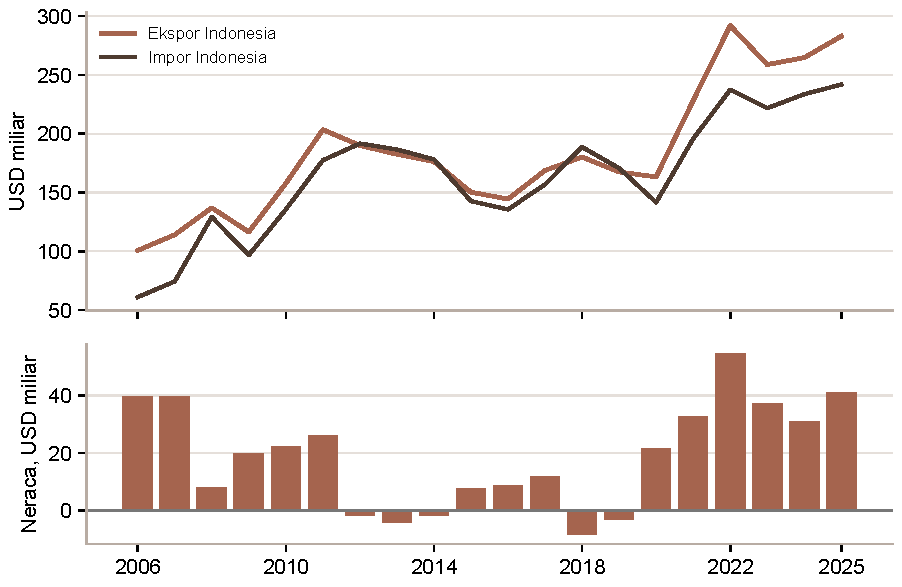
\includegraphics[width=\linewidth]{assets/indonesia_annual.pdf}
\caption{Ekspor, impor, dan trade balance Indonesia dengan seluruh negara. Grafik tahunan hanya memakai tahun dengan empat kuartal lengkap. Sumber: data Trade Map pengguna.}\label{fig:annual}
\end{figure}

\subsection{Mengapa ada tujuh kelompok barang?}
Ada dua cara pengelompokan yang dipakai. Cara pertama membedakan komoditas dari manufaktur nonkomoditas, mengikuti kelompok A11 UNCTAD melalui mapping HS--SITC \cite{unctad,unsdcorr}. Komoditas total kemudian dirinci menjadi pertanian/pangan dan energi/tambang.

Cara kedua melihat penggunaan barang: konsumsi, modal, atau bahan baku/penolong. Ini mengikuti BEC Rev.5 \cite{bec}. Kedua cara tersebut menjawab pertanyaan yang berbeda. Sebuah komoditas bisa menjadi barang konsumsi atau bahan baku. Barang manufaktur juga bisa menjadi barang modal atau input produksi.

\begin{table}[!htbp]\centering\small
\caption{Arti tujuh kelompok barang}
\begin{tabular}{p{.07\linewidth}p{.29\linewidth}p{.53\linewidth}}
\toprule Kode & Kelompok & Penjelasan\\\midrule
G1 & Manufaktur nonkomoditas & Barang nonkomoditas menurut mapping UNCTAD yang dipakai.\\
G2 & Barang konsumsi & Barang untuk konsumsi akhir menurut BEC Rev.5.\\
G3 & Pertanian dan pangan & Komoditas pangan dan bahan mentah pertanian.\\
G4 & Bahan baku/penolong & Barang untuk penggunaan antara dalam produksi.\\
G5 & Barang modal & Barang untuk pembentukan modal tetap.\\
G6 & Komoditas total & Semua komoditas A11 yang berhasil dipetakan.\\
G7 & Energi dan tambang & Bahan bakar, bijih/mineral, dan komoditas logam terkait.\\
\bottomrule\end{tabular}\label{tab:groups}
\end{table}

\textbf{Ketujuh kelompok tidak boleh dijumlahkan menjadi total perdagangan.} Sebagian nilainya masuk ke lebih dari satu kelompok karena cara pengelompokannya berbeda. Hasil regresi kelompok yang tumpang tindih juga tidak bisa dihitung sebagai bukti yang sepenuhnya independen.

Ada masalah lain yang belum selesai: workbook tidak menyebut versi HS untuk setiap angka. Kode yang sama bisa mempunyai mapping berbeda pada revisi yang berbeda. Karena itu, suatu kode hanya dimasukkan ke kelompok tertentu bila mapping resminya konsisten. Kode yang masih ambigu dibiarkan sebagai campuran atau belum terpetakan.

Nilai kode yang ambigu tetap masuk dalam TOTAL, tetapi tidak dipaksakan masuk ke kelompok yang belum jelas. Cara ini lebih hati-hati, namun belum membuat produk sepenuhnya sebanding dari tahun ke tahun. Hasil kelompok juga belum tentu berlaku untuk setiap produk atau perusahaan di dalamnya.

\subsection{Data GDP, kurs, dan harga}
Model memasukkan aktivitas ekonomi Indonesia dan negara mitra. Ukurannya adalah level \emph{real GDP}, atau PDB riil, yang diubah menjadi indeks lalu di-log. Ini berbeda dari memasukkan pertumbuhan GDP tahunan.

Untuk total perdagangan Indonesia, aktivitas luar negeri diwakili oleh gabungan real GDP sepuluh mitra dengan bobot ekspor tetap 2006--2008. Ini adalah proksi permintaan luar negeri. Angkanya tidak sama dengan GDP seluruh dunia.

Kurs total Indonesia menggunakan REER BIS. Kurs bilateral dibentuk dari kurs nominal dan indeks harga. Arahnya dibuat sama: angka kurs yang naik berarti apresiasi. Jadi, perubahan yang diuji adalah perubahan kurs riil, bukan otomatis perubahan rupiah terhadap dolar dengan besaran yang sama.

Indeks harga komoditas BCOM ditambahkan pada beberapa model pembanding. Tujuannya melihat apakah hasil berubah ketika satu ukuran harga global ikut dimasukkan. BCOM tidak langsung mengukur harga semua produk HS-6.

\subsection{Mengapa periode data tiap negara berbeda?}
Model hanya memakai rentang kuartal terpanjang yang lengkap. Jika ada kuartal kosong, kuartal sebelum dan sesudahnya tidak disambung seolah tidak ada jeda. Ini menjaga arti lag, yaitu jarak waktu dalam model.

Data CPI India yang dipakai baseline mulai 2013. CPI Australia bulanan memuat interpolasi dari penyedia. CPI AS Oktober 2025 dan kurs Vietnam Agustus 2025 kosong pada seri utama. Ada pula catatan tentang versi historis GDP dan perbedaan definisi kurs antarpenyedia. Karena itu, rentang estimasi tiap mitra tidak selalu sama.

Untuk total Indonesia, baseline dimulai dari data 2010Q1 agar bisa dibandingkan dengan run sebelumnya. Setelah empat lag disiapkan, regresinya memakai 2011Q1--2026Q1. Model dengan data mulai 2006 tetap dijalankan sebagai robustness check.

\begin{table}[!htbp]\centering\caption{Gambaran sampel total Indonesia, 2011Q1--2026Q1}
{\small\setlength{\tabcolsep}{3pt}\renewcommand{\arraystretch}{1.15}
\begin{tabular}{p{0.32\linewidth}p{0.045\linewidth}p{0.12\linewidth}p{0.12\linewidth}p{0.12\linewidth}p{0.12\linewidth}}
\toprule
\textbf{Variabel} & \textbf{N} & \textbf{Rerata} & \textbf{SD} & \textbf{Min.} & \textbf{Maks.}\\
\midrule
Ekspor, USD miliar & 61 & 51,15 & 12,46 & 33,60 & 78,20\\
Impor, USD miliar & 61 & 46,92 & 9,06 & 31,73 & 65,54\\
Neraca, USD miliar & 61 & 4,24 & 5,08 & -4,80 & 15,61\\
PDB riil Indonesia, indeks & 61 & 114,85 & 21,27 & 79,40 & 156,49\\
Aktivitas luar negeri, indeks & 61 & 109,43 & 13,98 & 86,16 & 135,66\\
REER, indeks & 61 & 100,99 & 4,32 & 92,89 & 111,01\\
\bottomrule
\end{tabular}
}\label{tab:desc}
\end{table}

Pada tabel ini, ekspor dan impor adalah nilai per kuartal. N berarti jumlah kuartal. SD adalah standard deviation, yaitu ukuran seberapa besar data bervariasi di sekitar rata-ratanya. Meski rata-rata trade balance positif, tetap ada kuartal defisit.

Perdagangan belum disesuaikan secara musiman. Sebagian GDP memakai seri penyedia yang sudah disesuaikan. Perbedaan ini masih perlu diperiksa dalam pengembangan model berikutnya.

\clearpage\section{Memahami model dan cara membaca hasilnya}\label{sec:methods}
\subsection{Apa yang sebenarnya diprediksi model?}
Trade balance dalam nilai dolar biasanya ditulis sebagai ekspor dikurangi impor. Untuk regresi, penelitian ini mengikuti paper acuan dan memakai log rasio impor terhadap ekspor:
\begin{equation}
 y_{s,t}=\ln\left(\frac{M_{s,t}}{X_{s,t}}\right),
 \qquad TB_{s,t}=X_{s,t}-M_{s,t}.\label{eq:outcome}
\end{equation}
$M$ adalah nilai impor Indonesia dan $X$ nilai ekspornya. Indeks $s$ menunjukkan cakupan, misalnya total Indonesia, Indonesia--Australia, atau komoditas Indonesia--Tiongkok. Indeks $t$ menunjukkan waktu.

Saat impor mengecil dibandingkan ekspor, rasio $M/X$ turun. Karena itu, penurunan $y$ berarti posisi perdagangan membaik. Rasio ini bisa digunakan untuk membandingkan pasar dengan ukuran perdagangan berbeda. Kedua arus harus positif agar log-nya dapat dihitung.

Trade balance dalam dolar tetap ditampilkan sebagai statistik deskriptif. Selisih dolar tidak di-log karena bisa bernilai negatif. Hasil regresi rasio juga tidak bisa langsung dibaca sebagai perubahan surplus dalam dolar.

\readingbox{\textbf{Contoh sederhana.} Jika ekspor turun 5\% dan impor turun 10\%, ekspor relatif terhadap impor justru membaik. Jadi, hasil model yang menunjukkan perbaikan rasio belum membuktikan bahwa ekspor meningkat.}

Nilai perdagangan juga memuat harga dan volume. Secara konsep, jika indeks harga dan volume dibentuk secara konsisten:
\begin{equation}
 \ln(M/X)=\ln P_M-\ln P_X+\ln Q_M-\ln Q_X.\label{eq:value}
\end{equation}
Persamaan ini membantu menjelaskan sumber perubahan nilai. Penelitian belum mengestimasi komponen tersebut secara terpisah karena belum memakai data kuantitas dan harga setiap produk.

\subsection{Kapan suatu respons disebut J-curve?}
Pola J berarti kondisi perdagangan memburuk lebih dahulu setelah depresiasi, lalu membaik. Salah satu kemungkinan penjelasannya adalah kontrak dan volume belum langsung menyesuaikan. Perbaikan baru terlihat setelah beberapa waktu.

Kurva yang langsung membaik tidak otomatis disebut J-curve. Kurva yang terlihat membentuk J pun masih perlu diperiksa confidence interval dan modelnya. Pada paper acuan, pembahasan ini menghubungkan respons jangka pendek dengan hubungan jangka panjang \cite{bahmani}.

Grafik penelitian ini berhenti pada kuartal ke-24, atau enam tahun setelah perubahan kurs. Titik terakhir grafik membantu membaca respons akhir periode, tetapi belum tentu persis sama dengan posisi long run yang sudah tercapai.

\subsection{ARDL: memasukkan pengaruh saat ini dan beberapa kuartal sebelumnya}
ARDL memakai nilai saat ini dan lag. Lag adalah nilai variabel pada periode sebelumnya. Misalnya, lag satu berarti satu kuartal sebelumnya. Dengan cara ini, model tidak memaksakan semua penyesuaian selesai pada kuartal yang sama.

Notasi dasarnya:
\begin{equation}
 y_t=a+\sum_{\ell=1}^{p}\phi_\ell y_{t-\ell}
       +\sum_{v\in\mathcal Z}\sum_{j=0}^{q_v}b_{v,j}v_{t-j}+\varepsilon_t,
 \qquad \mathcal Z=\{d,f,q\}.\label{eq:ardl}
\end{equation}
$d$ adalah log real GDP Indonesia, $f$ log aktivitas luar negeri, dan $q$ kurs riil. Rumus ini mengatakan bahwa rasio perdagangan sekarang dapat berkaitan dengan rasionya sendiri pada kuartal sebelumnya, aktivitas ekonomi, dan kurs pada beberapa periode.

Aktivitas Indonesia dimasukkan karena perubahan ekonomi domestik dapat memengaruhi kebutuhan impor sekaligus produksi. Aktivitas mitra membantu menangkap perubahan permintaan dari luar negeri. Tanda hasilnya tidak dipaksakan harus mengikuti satu dugaan.

Jika model stabil dan hubungan jangka panjangnya didukung, koefisien long run dihitung sebagai
\begin{equation}
 \beta_v=\frac{\sum_{j=0}^{q_v}b_{v,j}}{1-\sum_{\ell=1}^{p}\phi_\ell}.
 \label{eq:lr}
\end{equation}
ARDL memakai satu hubungan kurs untuk apresiasi dan depresiasi. Dengan kata lain, kedua arah dibatasi simetris dalam log. Ini berguna sebagai model pembanding yang lebih sederhana.

\subsection{NARDL: membedakan kurs menguat dan melemah}
NARDL memisahkan perubahan kurs positif dan negatif:
\begin{align}
 q_t^+&=\sum_{j=1}^{t}\max(\Delta q_j,0),&
 q_t^-&=\sum_{j=1}^{t}\min(\Delta q_j,0),\\
 q_t&=q_0+q_t^++q_t^-.
\end{align}
$\Delta q_t=q_t-q_{t-1}$ adalah perubahan kurs. Semua perubahan positif dijumlahkan ke $q^+$, sedangkan perubahan negatif dijumlahkan ke $q^-$. Ini disebut partial sums.

Dalam penelitian ini, kenaikan $q$ berarti apresiasi. Jadi, $q^+$ mewakili akumulasi penguatan dan $q^-$ akumulasi pelemahan. Nilai perubahan negatif tetap bertanda negatif, tidak diubah menjadi positif.

Regressor menjadi $\{d,f,q^+,q^-\}$. Untuk model pembanding harga, ditambahkan log BCOM. Pemisahan ini memungkinkan apresiasi dan depresiasi mempunyai hasil berbeda. Ia tidak sama dengan memasukkan volatilitas kurs sebagai variabel baru \cite{shin}.

\subsection{Apa fungsi error correction?}
Error correction membantu menghubungkan gerak jangka pendek dengan hubungan jangka panjang. Bentuk umum NARDL dapat ditulis:
\begin{align}
\Delta y_t={}&\alpha+\rho y_{t-1}+\theta_d d_{t-1}+\theta_f f_{t-1}
 +\theta_+q^+_{t-1}+\theta_-q^-_{t-1}\nonumber\\
 &+\sum_{j=1}^{P}\psi_j\Delta y_{t-j}
 +\sum_{j=0}^{Q_d}\gamma_{d,j}\Delta d_{t-j}
 +\sum_{j=0}^{Q_f}\gamma_{f,j}\Delta f_{t-j}\nonumber\\
 &+\sum_{j=0}^{Q_+}\pi_j^+\Delta q^+_{t-j}
 +\sum_{j=0}^{Q_-}\pi_j^-\Delta q^-_{t-j}+\eta_t.
 \label{eq:ecm}
\end{align}

Bagian dengan nilai periode sebelumnya membantu menjelaskan hubungan long run. Bagian dengan simbol $\Delta$ menjelaskan perubahan jangka pendek. Rumus ini menunjukkan bentuk umum; tidak semua suku harus bebas diestimasi pada setiap model. Itu bergantung pada lag yang terpilih.

Koefisien penyesuaian dan koefisien long run berhubungan melalui
\begin{equation}
 \rho=\sum_{\ell=1}^{p}\phi_\ell-1,\qquad
 \beta_-=-\theta_-/\rho,\qquad \beta_+=-\theta_+/\rho.
\end{equation}
Koefisien $\rho$ yang negatif sesuai dengan gagasan bahwa penyimpangan akan dikoreksi. Tetapi satu tanda negatif ini belum cukup untuk mengatakan bahwa seluruh hubungan long run sudah terbukti.

\subsection{Mengapa tanda koefisien bisa terasa terbalik?}
Pada total Indonesia dipakai $q=\ln(\mathrm{REER})$. Pada bilateral, tanda log RER dibalik agar arahnya sama: naik berarti apresiasi.

Depresiasi berarti perubahan negatif, $\delta^-<0$. Perubahan long run yang dihitung dari koefisien adalah
\begin{equation}
 \Delta y_\infty^-=\beta_-\delta^-.
\end{equation}
Jika $\beta_-$ positif, dikalikan perubahan kurs negatif hasilnya negatif. Karena $y$ adalah log impor/ekspor, hasil negatif berarti rasio perdagangan membaik. Jika koefisiennya negatif, arah hasilnya menjadi pemburukan.

Supaya grafik lebih mudah dibaca, tampilannya dibalik:
\begin{equation}
 R_h^J=-100\,\Delta_h y=100\,\Delta_h\ln(X/M).\label{eq:display}
\end{equation}
Dengan tampilan ini, positif selalu berarti perbaikan. Confidence interval ikut dibalik dengan cara yang sama. Angka hasil estimasi tidak berubah; yang berubah hanya arah penyajian.

Besarnya perubahan kurs yang digunakan adalah $-\ln(1.10)$ untuk depresiasi dan $+\ln(1.10)$ untuk apresiasi. Keduanya sama besar dalam log. Dalam persen biasa, ini berarti penurunan sekitar 9,09\% dan kenaikan 10\%.

\subsection{Apa yang dipakai untuk mewakili permintaan luar negeri?}
Model bilateral memakai real GDP mitra. Model total Indonesia memakai gabungan sepuluh mitra:
\begin{equation}
 f_t=\ln\left(\sum_{i=1}^{10}w_iY^{(2015=100)}_{i,t}\right),
 \qquad \sum_{i=1}^{10}w_i=1.
\end{equation}
$w_i$ adalah bobot berdasarkan pangsa ekspor 2006--2008. GDP tiap mitra diubah menjadi indeks agar tidak menjumlahkan angka uang dari mata uang yang berbeda.

Proksi ini mempunyai keterbatasan. Negara di luar sepuluh mitra tidak terwakili langsung, dan bobot tetap tidak mengikuti perubahan pangsa ekspor. Karena itu, hasil total Indonesia tetap bergantung pada cara permintaan luar negeri diukur.

\subsection{Bagaimana lag dipilih?}
Model mencoba beberapa pilihan lag lalu memakai AIC untuk memilih. AIC mempertimbangkan kecocokan model sekaligus memberi penalti jika parameter bertambah:
\begin{equation}
 \mathrm{AIC}=N\ln(\mathrm{RSS}/N)+2K,\qquad
 \mathrm{BIC}=N\ln(\mathrm{RSS}/N)+K\ln N.
\end{equation}
$N$ adalah jumlah kuartal dan $K$ jumlah parameter. RSS merangkum besarnya residual. Residual adalah selisih angka aktual dengan angka yang diperkirakan model.

Maksimum lag level pada model utama adalah empat. Maksimum dua digunakan sebagai robustness check, yaitu pemeriksaan apakah hasil berubah saat pilihan model diubah. ARDL dan NARDL pada batas lag yang sama memakai awal sampel efektif yang sama.

Mengurangi maksimum lag menjadi dua bisa menambah dua kuartal awal ke sampel. Jadi, pembanding ini mengubah lag dan sedikit mengubah periode data. Ia belum menjadi perbandingan lag pada sampel yang benar-benar identik.

Paper acuan memakai maksimum delapan lag first difference pada sampel yang lebih panjang. Empat lag level di sini adalah penyesuaian untuk data Indonesia, bukan padanan persis delapan lag first difference.

\subsection{Kapan hasil boleh dibaca sebagai hubungan long run?}
Bounds test membantu memeriksa apakah model memberi bukti hubungan jangka panjang \cite{pss,ks}. Run ini memakai statistik F dan t serta p-value finite-sample dari implementasi Stata. Keputusan utama memakai ambang 5\% untuk keduanya.

Ada pemeriksaan tambahan. Joint-X test melihat apakah variabel penjelas dalam bentuk level bersama-sama ikut mendukung hubungan itu. Model juga diperiksa dari kestabilan dinamika, sifat time series, dan sisa derajat bebas. Dalam run ini, minimal sisa derajat bebas adalah 15.

Sifat time series diperiksa dengan unit root tests ADF dan PP. Secara sederhana, ini berkaitan dengan apakah sifat statistik seri sudah stabil atau perlu diambil perubahannya. ARDL bounds dirancang untuk kombinasi $I(0)$ dan $I(1)$, bukan variabel $I(2)$.

ADF memilih lag melalui BIC pada nol sampai empat; PP memakai empat lag. Jika keduanya gagal menolak unit root pada first difference di ambang 10\%, run memberi catatan risiko $I(2)$. Catatan ini belum membuktikan bahwa variabel benar-benar $I(2)$; sampel kecil juga bisa membuat tes kurang kuat.

Paper acuan membahas pula beberapa hasil pada 10\%. Run ini menyimpan keputusan F-only 10\% sebagai pembanding. Kesimpulan utama tetap memakai F dan t 5\% beserta pemeriksaan tambahan, sehingga kriterianya lebih ketat daripada sebagian pembacaan dalam paper acuan.

\subsection{P-value, confidence interval, dan asymmetry}
P-value membantu menilai seberapa jauh data bertentangan dengan hipotesis nol di bawah asumsi model. P-value kecil bukan berarti kita sudah mengetahui peluang hipotesis itu benar atau salah.

Confidence interval menunjukkan ketidakpastian di sekitar koefisien atau respons. Interval yang lebar bisa mencakup kemungkinan pengaruh negatif maupun positif. Jadi, hasil yang tidak signifikan belum membuktikan bahwa pengaruhnya nol.

Asymmetry berarti apresiasi dan depresiasi bisa mempunyai koefisien berbeda. Uji Wald long run memeriksa $H_0:\beta_+=\beta_-$. Untuk jangka pendek, pembandingnya memakai jumlah koefisien perubahan. Asymmetry yang signifikan belum menggantikan bounds test; kedua tes menilai hal berbeda.

Dynamic multipliers menunjukkan bagaimana respons berubah menurut waktu:
\begin{equation}
 m_h^\pm=\frac{\partial y_{t+h}}{\partial q_t^\pm},\qquad
 R_h^{J,\pm}=-100\,m_h^\pm\delta^\pm,\qquad h=0,\ldots,24.
\end{equation}
Confidence interval 95\% dihitung dengan delta method dan kuantil t dari model. Intervalnya pointwise: berlaku pada tiap horizon, bukan jaminan 95\% untuk seluruh jalur sekaligus.

AIC sudah dipakai untuk memilih model sebelum p-value dan interval dihitung. Angka tersebut belum mengoreksi ketidakpastian pemilihan model. BH \cite{bh} juga dilaporkan untuk mengurangi risiko pembacaan terlalu optimistis ketika banyak koefisien diuji. BH diterapkan dalam kelompok pengujian tertentu: satu model total, sepuluh bilateral, dan 77 model barang per estimator. Ini belum menjadi koreksi lengkap seluruh pencarian 516 model.

\readingbox{\textbf{Cara membaca satu hasil.} Mulai dari arah koefisien, lihat confidence interval, cek hubungan long run, lalu baca diagnostic tests dan robustness checks. Jangan mengambil kesimpulan hanya dari satu p-value atau bentuk garis.}

\clearpage\section{Hasil untuk total perdagangan Indonesia}\label{sec:aggregate}
\subsection{Bukti long run masih belum cukup}
Model total Indonesia memakai ekspor ke seluruh negara dan impor dari seluruh negara. Sampel utamanya berisi 61 kuartal, yaitu 2011Q1--2026Q1.

ARDL memilih lag $(2,3,0,4)$. Urutannya adalah rasio perdagangan, GDP Indonesia, aktivitas luar negeri, dan kurs. NARDL memilih $(2,0,3,0,4)$, dengan dua angka terakhir untuk partial sums apresiasi dan depresiasi. Ini pilihan AIC dari kandidat yang tersedia, bukan kepastian bahwa proses ekonomi mempunyai lag persis seperti itu.

\begin{table}[!htbp]\centering\caption{Bounds test untuk total perdagangan Indonesia}
{\small\setlength{\tabcolsep}{3pt}\renewcommand{\arraystretch}{1.15}
\begin{tabular}{p{0.1\linewidth}p{0.08\linewidth}p{0.08\linewidth}p{0.1\linewidth}p{0.1\linewidth}p{0.12\linewidth}p{0.22\linewidth}}
\toprule
\textbf{Model} & \textbf{F} & \textbf{t} & \textbf{p F(I1)} & \textbf{p t(I1)} & \textbf{p joint-X} & \textbf{Keputusan}\\
\midrule
ARDL & 2,481 & -2,280 & 0,369 & 0,434 & 0,259 & No rejection\\
NARDL & 3,799 & -2,887 & 0,094 & 0,279 & 0,011 & Inconclusive\\
\bottomrule
\end{tabular}
}\label{tab:worldbounds}
\end{table}

Pada ARDL, koefisien kurs sekitar 0,429 dengan p-value 0,661. Confidence interval melewati nol, dan bounds test belum mendukung hubungan long run. Diagnostic tests tidak menemukan masalah pada pemeriksaan yang dipakai, tetapi itu belum mengubah hasil bounds test.

Pada NARDL, koefisien depresiasi sekitar 2,572 dengan p-value 0,040. Koefisien apresiasi sekitar $-2,142$, sedangkan p-value uji asymmetry sekitar 0,006. Jika hanya angka ini yang dilihat, hasilnya tampak mendukung perbaikan saat rupiah melemah.

Tetapi p-value upper bound untuk F sekitar 0,094 dan untuk t sekitar 0,279. Keduanya belum memenuhi aturan utama 5\%. CUSUMSQ juga memberi catatan stabilitas. Jadi, signifikansi satu koefisien belum cukup untuk menyimpulkan adanya hubungan long run yang kuat.

\begin{figure}[!htbp]\centering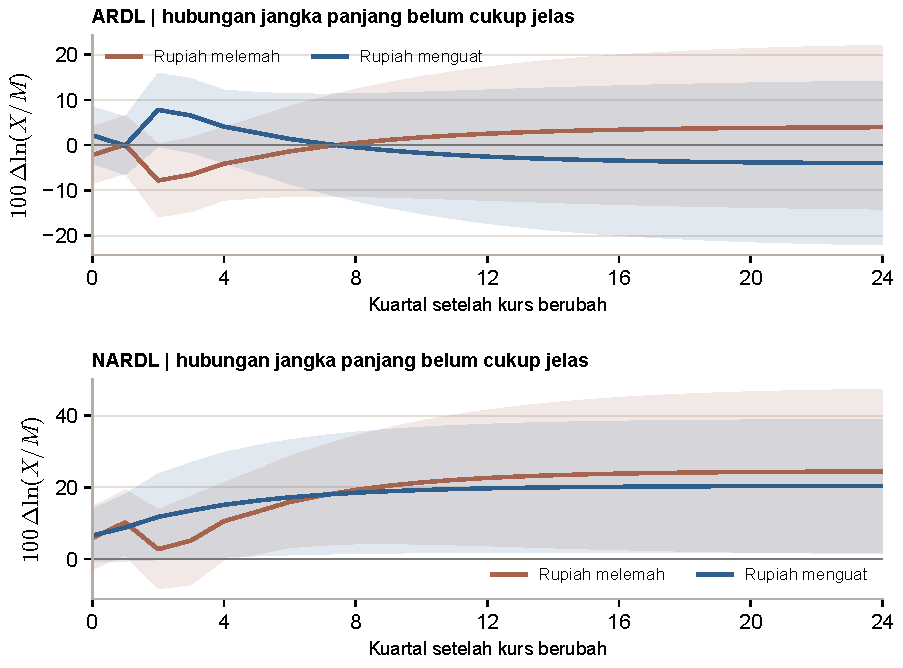
\includegraphics[width=\linewidth]{assets/response_WORLD.pdf}
\caption{Respons total perdagangan Indonesia. Cokelat: rupiah melemah; biru: rupiah menguat. Area berwarna adalah confidence interval 95\% per horizon. Positif berarti rasio ekspor/impor membaik.}\label{fig:world}
\end{figure}

\subsection{Apa yang bisa dibaca dari grafik?}
Garis utama ARDL memburuk dahulu lalu membaik. Tetapi confidence interval-nya cukup lebar dan masih mencakup nol pada bagian penting jalur. NARDL lebih banyak mengarah pada perbaikan, dengan fluktuasi pada awal periode.

Grafik membantu memahami jalur yang dihasilkan model. Namun bentuk yang terlihat baik belum menyelesaikan masalah pada bounds test dan stabilitas. Model utama masih belum memberikan dasar long run yang kuat.

Pada NARDL, kedua arah kurs bisa sama-sama terlihat memperbaiki rasio. Ini muncul dari tanda koefisien apresiasi dan depresiasi. Hasil tersebut belum bisa dibaca sebagai saran bahwa rupiah menguat maupun melemah pasti sama-sama menguntungkan. Model merangkum pengalaman historis dan perubahan lain yang bergerak bersama kurs.

Baseline mulai 2010 dipakai agar bisa dibandingkan dengan run sebelumnya. Data mulai 2006 juga dijalankan sebagai robustness check. Kita tidak memilih periode hanya karena tandanya lebih sesuai harapan.

\subsection{Contoh: apa arti koefisien 3,356?}
Contoh Australia lebih mudah dipakai karena NARDL-nya lolos pemeriksaan utama. Koefisien depresiasinya $\widehat{\beta}_-=\AusBetaMath$. Jika perubahan log kurs sebesar $-\ln(1.10)$, respons long run yang ditampilkan adalah
\begin{equation}
 -100\,\widehat{\beta}_-\big[-\ln(1.10)\big]\simeq\AusResponseMath.
\end{equation}
Angka \AusResponse{} adalah \textbf{poin log kali seratus}, bukan kenaikan surplus dolar sebesar \AusResponse\%. Untuk mengubahnya menjadi perubahan persentase rasio ekspor/impor, rumusnya:
\begin{equation}
 100\left[\exp\{-\widehat{\beta}_-\delta^-\}-1\right].
\end{equation}
Hasilnya sekitar \AusRatioPct\%. Ini tetap perubahan rasio ekspor/impor yang dihitung dari model. Angkanya belum berarti ekspor naik \AusRatioPct\% dan belum menjadi ramalan kebijakan yang pasti.

Koefisien, poin log, persentase rasio, dan perubahan surplus dolar adalah empat hal yang berbeda. Semuanya tetap bergantung pada asumsi dan ketidakpastian model asalnya.

\clearpage\section{Hasil tiap mitra}\label{sec:bilateral}

\subsection{Gambaran umumnya}

Hasil total tiap mitra berbeda. Australia dan Malaysia memberi NARDL yang lebih mendukung, tetapi signifikansi Malaysia lebih lemah setelah BH. Model lain tetap ditampilkan, termasuk yang mempunyai koefisien besar atau p-value kecil tetapi belum lolos pemeriksaan long run.

\begin{table}[!htbp]\centering\caption{Ringkasan NARDL Indonesia dengan sepuluh mitra}{\small\setlength{\tabcolsep}{3pt}\renewcommand{\arraystretch}{1.15}
\begin{tabular}{p{0.17\linewidth}p{0.045\linewidth}p{0.2\linewidth}p{0.12\linewidth}p{0.09\linewidth}p{0.09\linewidth}p{0.07\linewidth}}
\toprule
\textbf{Mitra} & \textbf{N} & \textbf{Rentang} & \textbf{Koef. dep.} & \textbf{p} & \textbf{BH} & \textbf{Status}\\
\midrule
Australia & 77 & 2007Q1--2026Q1 & 3,356 & \(<0{,}001\) & 0,004 & L+D\\
Tiongkok & 78 & 2007Q1--2026Q2 & -2,727 & 0,250 & 0,350 & --\\
India & 49 & 2014Q1--2026Q1 & -6,443 & 0,236 & 0,350 & --\\
Jepang & 78 & 2007Q1--2026Q2 & -2,456 & 0,006 & 0,020 & --\\
Korea Selatan & 78 & 2007Q1--2026Q2 & 3,935 & 0,144 & 0,288 & --\\
Malaysia & 78 & 2007Q1--2026Q2 & 1,346 & 0,024 & 0,059 & L+D\\
Singapura & 78 & 2007Q1--2026Q2 & -0,262 & 0,810 & 0,810 & --\\
Thailand & 78 & 2007Q1--2026Q2 & 0,950 & 0,280 & 0,350 & L\\
Amerika Serikat & 75 & 2007Q1--2025Q3 & 3,095 & 0,006 & 0,020 & --\\
Vietnam & 74 & 2007Q1--2025Q2 & -0,551 & 0,737 & 0,810 & --\\
\bottomrule
\end{tabular}
}\label{tab:bilateral}\end{table}

\begin{figure}[!htbp]\centering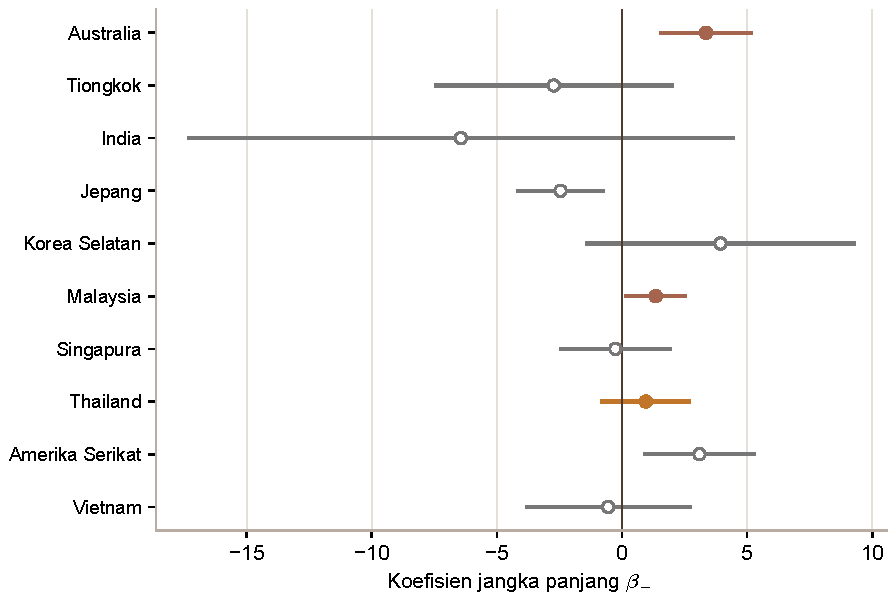
\includegraphics[width=\linewidth]{assets/bilateral_forest.pdf}\caption{Koefisien depresiasi NARDL. Cokelat: long run dan diagnostic tests terpenuhi; emas: ada catatan model; simbol kosong: bukti long run belum cukup.}\label{fig:bilateralforest}\end{figure}


Periode data tiap mitra tidak sama. Karena itu, perbedaan koefisien belum menjadi uji formal bahwa negara-negara tersebut mempunyai efek yang berbeda.

\clearpage\subsection{Indonesia--Australia}

Australia termasuk hasil yang lebih mendukung perbaikan rasio perdagangan saat rupiah melemah. ARDL dan NARDL sama-sama lolos pemeriksaan utama. Pada NARDL, signifikansi koefisien depresiasi juga bertahan setelah BH.

Garis NARDL memburuk dahulu lalu membaik, sehingga ada pola J pada garis utama. Tetapi confidence interval awal masih melewati nol. Jadi, pemburukan awalnya belum sekuat kepastian yang terlihat dari garis saja. Uji asymmetry juga belum menolak kesamaan kedua arah kurs pada 5\%.

\noindent\textbf{Angka utamanya.} NARDL memakai 77 kuartal pada 2007Q1--2026Q1. Koefisien depresiasi 3,356, confidence interval 95\% [1,563; 5,149], p-value \(<0{,}001\), dan BH 0,004. P-value asymmetry 0,147.

\noindent\textbf{Catatan pemeriksaan.} tidak ada masalah yang terdeteksi pada pemeriksaan yang dipakai.

\begin{figure}[!htbp]\centering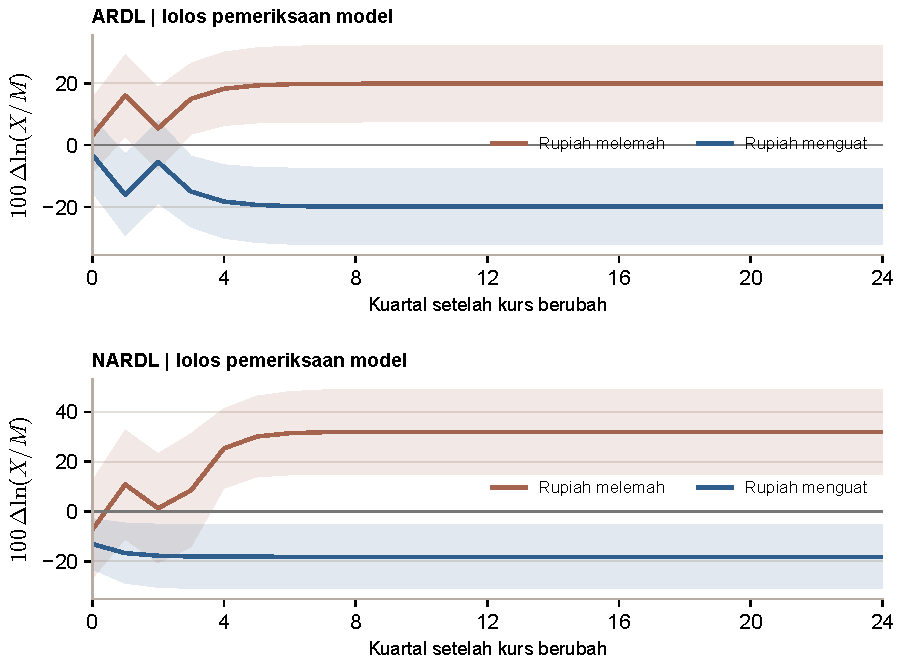
\includegraphics[width=\linewidth]{assets/response_BIL_AUS.pdf}\caption{Respons perdagangan Indonesia--Australia. Positif berarti rasio ekspor/impor membaik. Confidence interval berlaku per horizon; skala panel berbeda.}\label{fig:bilAUS}\end{figure}


\clearpage\subsection{Indonesia--Tiongkok}

Besarnya perdagangan dengan Tiongkok belum membuat hasil modelnya lebih pasti. Kedua model total bilateral belum lolos pemeriksaan long run. NARDL mempunyai catatan autocorrelation, sedangkan ARDL mendapat catatan CUSUM.

Karena itu, tanda negatif belum cukup untuk menyimpulkan bahwa depresiasi merugikan seluruh perdagangan Indonesia dengan Tiongkok. Kelompok pertanian nantinya memberi hasil yang berbeda dan lebih mendukung. Defisit bilateral pada data tahunan juga belum membuktikan bahwa kurs adalah penyebabnya.

\noindent\textbf{Angka utamanya.} NARDL memakai 78 kuartal pada 2007Q1--2026Q2. Koefisien depresiasi -2,727, confidence interval 95\% [-7,427; 1,972], p-value 0,250, dan BH 0,350. P-value asymmetry 0,905.

\noindent\textbf{Catatan pemeriksaan.} bounds test belum memberi bukti yang cukup; joint-X test belum mendukung; ada catatan pada residual atau stabilitas model.

\begin{figure}[!htbp]\centering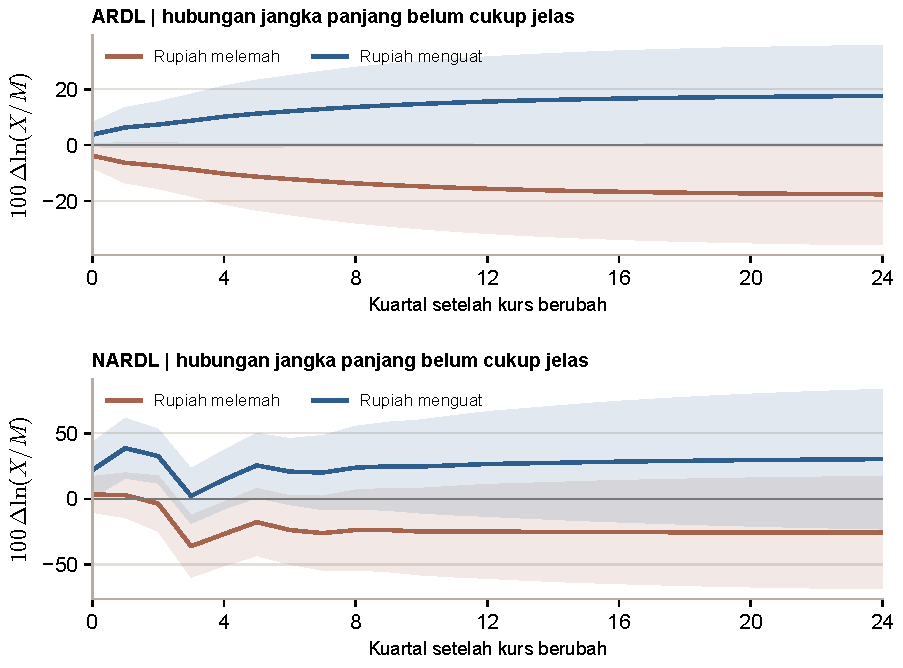
\includegraphics[width=\linewidth]{assets/response_BIL_CHN.pdf}\caption{Respons perdagangan Indonesia--Tiongkok. Positif berarti rasio ekspor/impor membaik. Confidence interval berlaku per horizon; skala panel berbeda.}\label{fig:bilCHN}\end{figure}


\clearpage\subsection{Indonesia--India}

India mempunyai data lebih pendek karena baseline memakai CPI mulai 2013. Dengan lebih banyak parameter pada NARDL, informasi untuk masing-masing angka menjadi terbatas. Koefisien depresiasinya negatif, tetapi confidence interval lebar dan bounds test belum mendukung long run.

Uji asymmetry signifikan, tetapi itu belum menyelesaikan persoalan bounds test. Diagnostic tests NARDL tidak menemukan masalah yang diperiksa, sedangkan ARDL mempunyai catatan autocorrelation dan RESET. WPI hanya dipakai sebagai pembanding terpisah, bukan dianggap CPI yang sama.

\noindent\textbf{Angka utamanya.} NARDL memakai 49 kuartal pada 2014Q1--2026Q1. Koefisien depresiasi -6,443, confidence interval 95\% [-17,300; 4,414], p-value 0,236, dan BH 0,350. P-value asymmetry 0,021.

\noindent\textbf{Catatan pemeriksaan.} bounds test belum memberi bukti yang cukup; joint-X test belum mendukung.

\begin{figure}[!htbp]\centering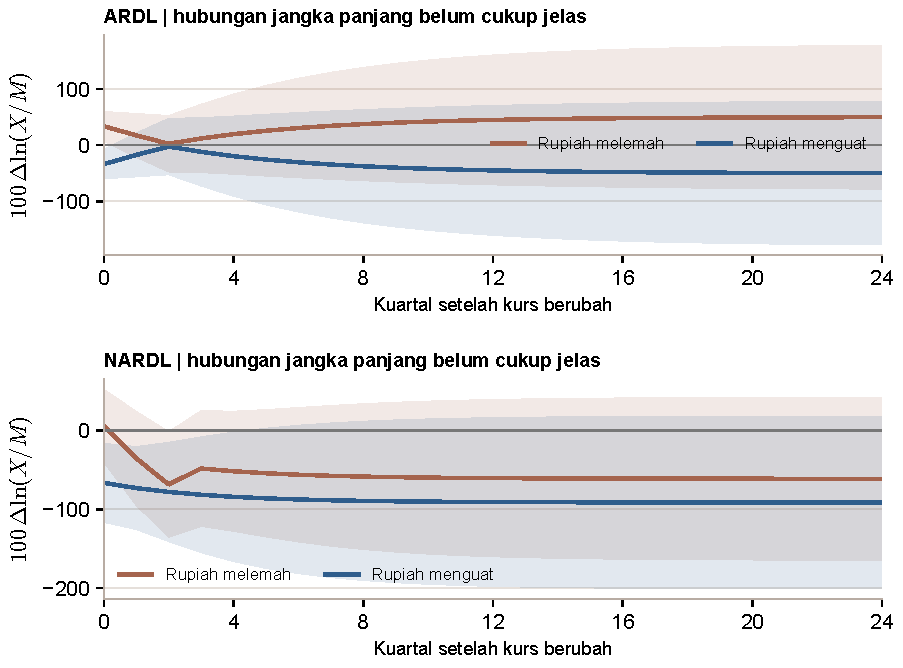
\includegraphics[width=\linewidth]{assets/response_BIL_IND.pdf}\caption{Respons perdagangan Indonesia--India. Positif berarti rasio ekspor/impor membaik. Confidence interval berlaku per horizon; skala panel berbeda.}\label{fig:bilIND}\end{figure}


\clearpage\subsection{Indonesia--Jepang}

Jepang memberi contoh mengapa p-value koefisien tidak boleh dibaca sendirian. Koefisien depresiasi NARDL negatif dan signifikan, termasuk setelah BH. Tetapi F bounds dan t bounds belum sama-sama memenuhi aturan 5\%.

Ada pula catatan ARCH dan normality test. Jadi, hasil ini tetap dilaporkan tetapi belum dipakai sebagai kesimpulan long run yang kuat. Tanda negatifnya adalah temuan yang perlu ditinjau lebih lanjut, bukan bukti pasti bahwa ekspor Indonesia ke Jepang turun karena depresiasi.

\noindent\textbf{Angka utamanya.} NARDL memakai 78 kuartal pada 2007Q1--2026Q2. Koefisien depresiasi -2,456, confidence interval 95\% [-4,166; -0,747], p-value 0,006, dan BH 0,020. P-value asymmetry 0,971.

\noindent\textbf{Catatan pemeriksaan.} bounds test belum memberi bukti yang cukup; ada catatan pada residual atau stabilitas model.

\begin{figure}[!htbp]\centering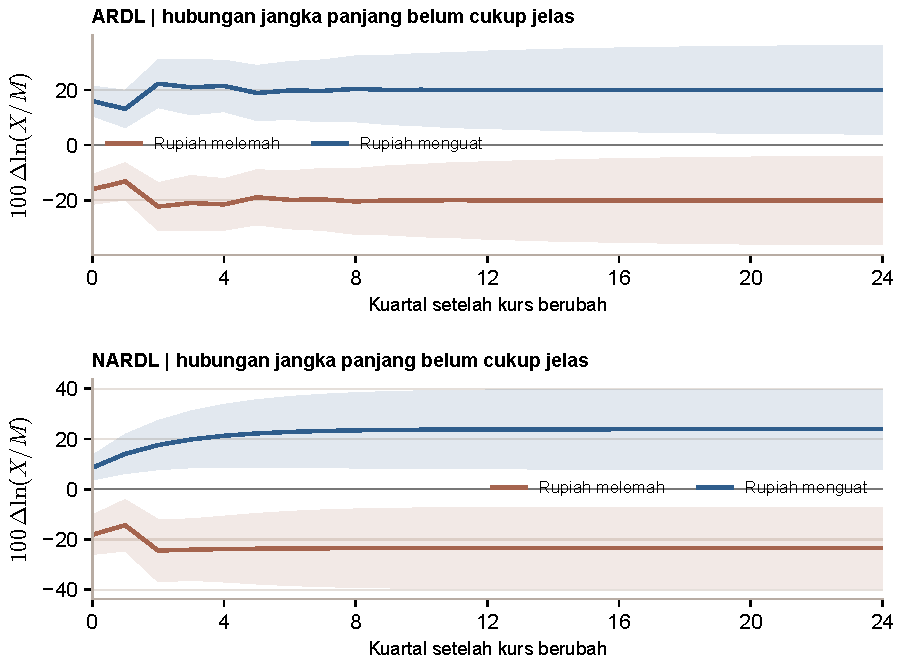
\includegraphics[width=\linewidth]{assets/response_BIL_JPN.pdf}\caption{Respons perdagangan Indonesia--Jepang. Positif berarti rasio ekspor/impor membaik. Confidence interval berlaku per horizon; skala panel berbeda.}\label{fig:bilJPN}\end{figure}


\clearpage\subsection{Indonesia--Korea Selatan}

Koefisien depresiasi NARDL Korea positif, tetapi cukup tidak pasti. Pemeriksaan long run belum lengkap, dan ada catatan autocorrelation, RESET, serta CUSUM. ARDL lebih dekat ke nol, tetapi juga belum mendukung long run.

Pada kelompok modal, hasil NARDL justru lebih mendukung dan pola J lebih jelas. Ini memperlihatkan bahwa hasil total mitra bisa menutupi kelompok tertentu. Namun barang modal tetap hanya sebagian perdagangan Indonesia dengan Korea.

\noindent\textbf{Angka utamanya.} NARDL memakai 78 kuartal pada 2007Q1--2026Q2. Koefisien depresiasi 3,935, confidence interval 95\% [-1,383; 9,253], p-value 0,144, dan BH 0,288. P-value asymmetry 0,112.

\noindent\textbf{Catatan pemeriksaan.} bounds test belum memberi bukti yang cukup; joint-X test belum mendukung; ada catatan pada residual atau stabilitas model.

\begin{figure}[!htbp]\centering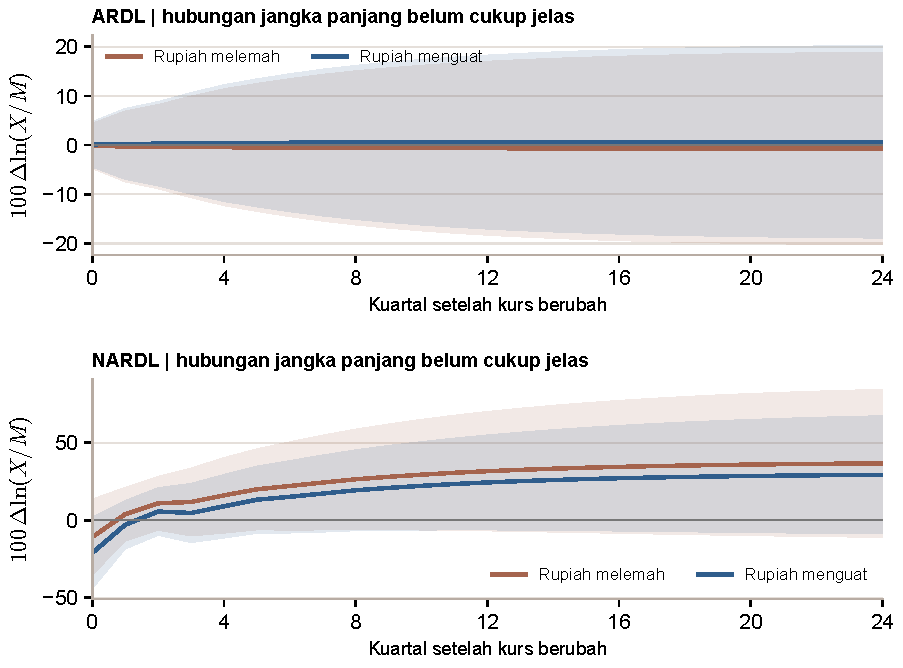
\includegraphics[width=\linewidth]{assets/response_BIL_KOR.pdf}\caption{Respons perdagangan Indonesia--Korea Selatan. Positif berarti rasio ekspor/impor membaik. Confidence interval berlaku per horizon; skala panel berbeda.}\label{fig:bilKOR}\end{figure}


\clearpage\subsection{Indonesia--Malaysia}

Malaysia memperlihatkan perbedaan ARDL dan NARDL yang cukup besar. ARDL mendukung long run, tetapi koefisien kursnya negatif, tidak signifikan pada 5\%, dan ada catatan RESET serta CUSUM. NARDL memberi koefisien depresiasi positif dan lolos pemeriksaan utama.

P-value depresiasi NARDL sekitar 0,024, tetapi setelah BH sekitar 0,059. Jadi, signifikansinya tidak bertahan pada ambang 5\% setelah koreksi tersebut. Kurva yang membaik juga belum tentu J-curve jika tidak mempunyai fase awal memburuk.

\noindent\textbf{Angka utamanya.} NARDL memakai 78 kuartal pada 2007Q1--2026Q2. Koefisien depresiasi 1,346, confidence interval 95\% [0,186; 2,507], p-value 0,024, dan BH 0,059. P-value asymmetry \(<0{,}001\).

\noindent\textbf{Catatan pemeriksaan.} tidak ada masalah yang terdeteksi pada pemeriksaan yang dipakai.

\begin{figure}[!htbp]\centering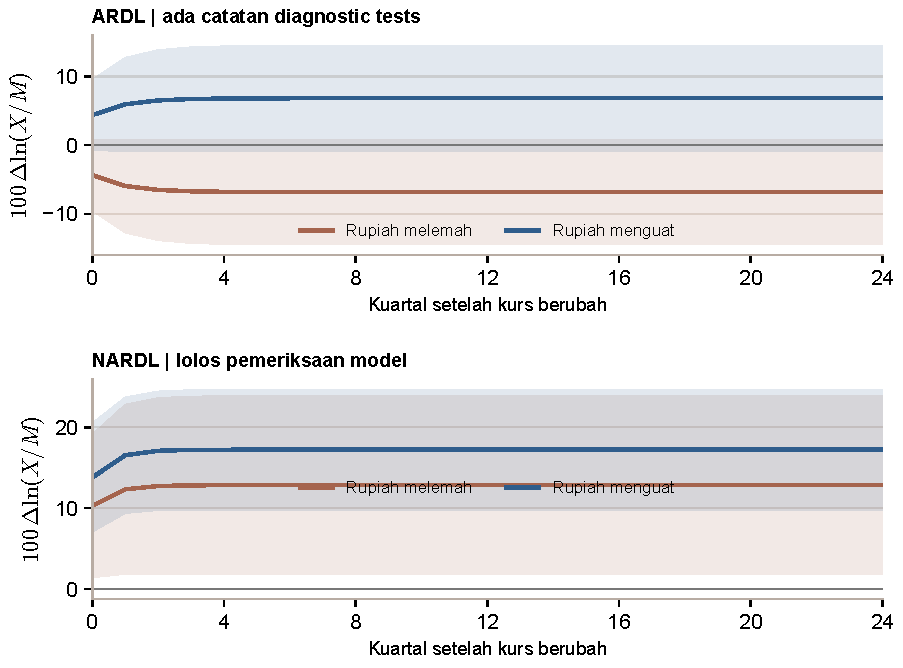
\includegraphics[width=\linewidth]{assets/response_BIL_MYS.pdf}\caption{Respons perdagangan Indonesia--Malaysia. Positif berarti rasio ekspor/impor membaik. Confidence interval berlaku per horizon; skala panel berbeda.}\label{fig:bilMYS}\end{figure}


\clearpage\subsection{Indonesia--Singapura}

Pada Singapura, F dan t bounds dapat menolak sementara joint-X test belum mendukung. Artinya, aturan lengkap untuk membaca long run belum terpenuhi. ARDL menunjukkan bahwa diagnostic tests yang tidak menemukan masalah belum cukup jika pemeriksaan long run lainnya belum lolos.

Koefisien depresiasi NARDL dekat nol pada garis utama, tetapi intervalnya tetap perlu dilihat. Kita belum bisa menyebutnya tidak sensitif karena belum ada uji khusus untuk memastikan efeknya kecil.

\noindent\textbf{Angka utamanya.} NARDL memakai 78 kuartal pada 2007Q1--2026Q2. Koefisien depresiasi -0,262, confidence interval 95\% [-2,440; 1,915], p-value 0,810, dan BH 0,810. P-value asymmetry 0,791.

\noindent\textbf{Catatan pemeriksaan.} joint-X test belum mendukung; ada catatan pada residual atau stabilitas model.

\begin{figure}[!htbp]\centering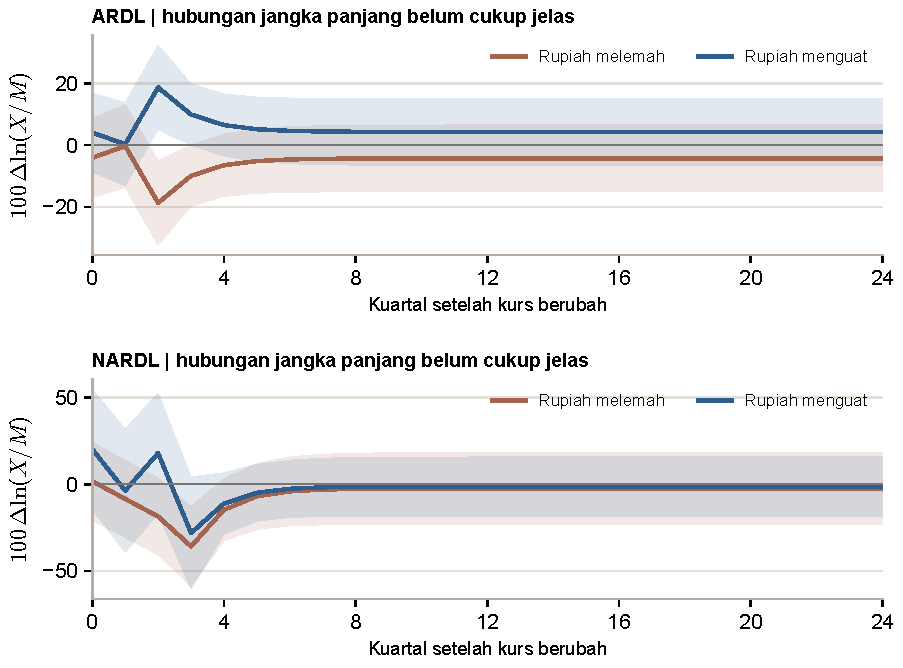
\includegraphics[width=\linewidth]{assets/response_BIL_SGP.pdf}\caption{Respons perdagangan Indonesia--Singapura. Positif berarti rasio ekspor/impor membaik. Confidence interval berlaku per horizon; skala panel berbeda.}\label{fig:bilSGP}\end{figure}


\clearpage\subsection{Indonesia--Thailand}

Thailand mempunyai dukungan long run pada kedua model. Tetapi ARCH dan CUSUMSQ memberi catatan, dengan tambahan CUSUM pada NARDL. Koefisien depresiasi NARDL juga belum signifikan.

Kurs Thailand mempunyai catatan perbedaan definisi antarpenyedia. Seri GEM dipakai sebagai robustness check secara penuh, bukan untuk menambal satu angka baseline. Perbandingan sumber perlu memperhatikan definisi dan periode data. Hasilnya belum menjadi efek kebijakan yang pasti stabil.

\noindent\textbf{Angka utamanya.} NARDL memakai 78 kuartal pada 2007Q1--2026Q2. Koefisien depresiasi 0,950, confidence interval 95\% [-0,789; 2,690], p-value 0,280, dan BH 0,350. P-value asymmetry 0,765.

\noindent\textbf{Catatan pemeriksaan.} ada catatan pada residual atau stabilitas model.

\begin{figure}[!htbp]\centering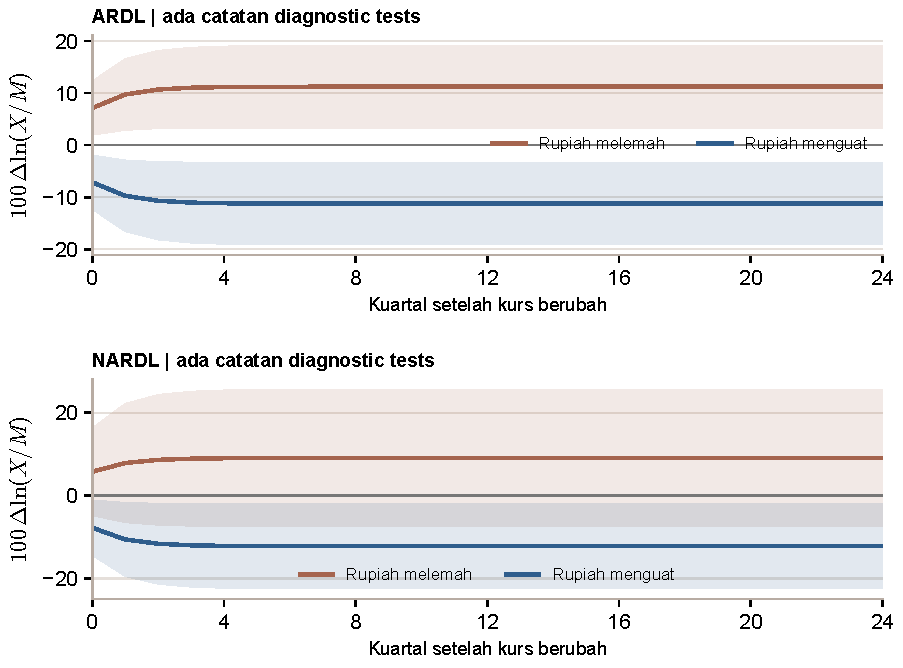
\includegraphics[width=\linewidth]{assets/response_BIL_THA.pdf}\caption{Respons perdagangan Indonesia--Thailand. Positif berarti rasio ekspor/impor membaik. Confidence interval berlaku per horizon; skala panel berbeda.}\label{fig:bilTHA}\end{figure}


\clearpage\subsection{Indonesia--Amerika Serikat}

Koefisien depresiasi NARDL AS positif dan signifikan, termasuk setelah BH. F dan t bounds juga menolak. Tetapi joint-X sekitar 0,060 belum memenuhi ambang 5\%, sehingga aturan long run lengkap belum terpenuhi. Ada pula catatan CUSUMSQ dan normality test.

Sampel utama berhenti pada 2025Q3 karena CPI Oktober 2025 kosong pada seri yang dipakai. Kelompok konsumsi dengan AS memberi hasil berbeda dan pola J lebih jelas. Itu belum memperbaiki kelemahan model total karena barang yang dihitung berbeda.

\noindent\textbf{Angka utamanya.} NARDL memakai 75 kuartal pada 2007Q1--2025Q3. Koefisien depresiasi 3,095, confidence interval 95\% [0,921; 5,269], p-value 0,006, dan BH 0,020. P-value asymmetry 0,240.

\noindent\textbf{Catatan pemeriksaan.} joint-X test belum mendukung; ada catatan pada residual atau stabilitas model.

\begin{figure}[!htbp]\centering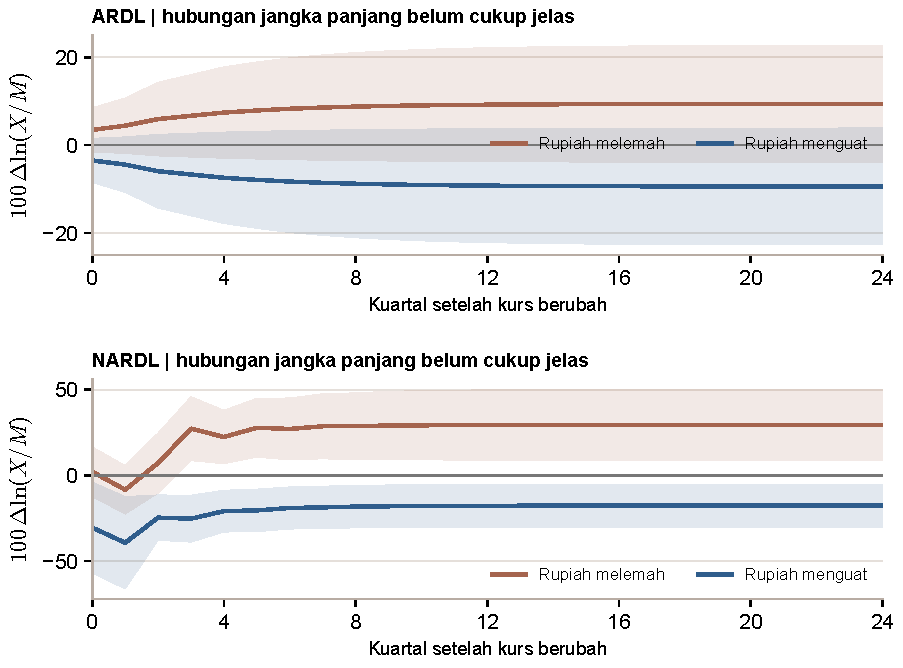
\includegraphics[width=\linewidth]{assets/response_BIL_USA.pdf}\caption{Respons perdagangan Indonesia--Amerika Serikat. Positif berarti rasio ekspor/impor membaik. Confidence interval berlaku per horizon; skala panel berbeda.}\label{fig:bilUSA}\end{figure}


\clearpage\subsection{Indonesia--Vietnam}

Vietnam mempunyai beberapa catatan variasi residual dan stabilitas. Koefisien depresiasi NARDL negatif dan tidak signifikan. T bounds juga belum mendukung long run. ARDL pun belum lolos pemeriksaan lengkap.

Kurs Agustus 2025 yang kosong membuat rentang utama berakhir pada 2025Q2. Kuartal setelah celah tidak disambung seolah tidak ada jeda. Alternatif GEM menjadi robustness check tersendiri. Keterbatasan ini perlu diingat saat membandingkan Vietnam dengan negara yang datanya berakhir lebih akhir.

\noindent\textbf{Angka utamanya.} NARDL memakai 74 kuartal pada 2007Q1--2025Q2. Koefisien depresiasi -0,551, confidence interval 95\% [-3,806; 2,704], p-value 0,737, dan BH 0,810. P-value asymmetry 0,163.

\noindent\textbf{Catatan pemeriksaan.} bounds test belum memberi bukti yang cukup; ada catatan pada residual atau stabilitas model.

\begin{figure}[!htbp]\centering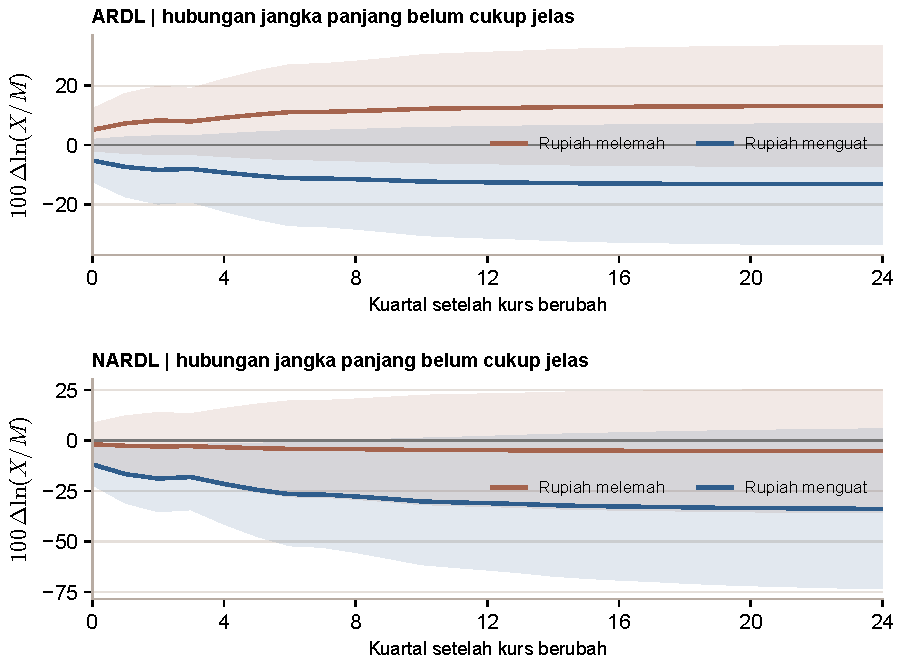
\includegraphics[width=\linewidth]{assets/response_BIL_VNM.pdf}\caption{Respons perdagangan Indonesia--Vietnam. Positif berarti rasio ekspor/impor membaik. Confidence interval berlaku per horizon; skala panel berbeda.}\label{fig:bilVNM}\end{figure}

\clearpage\section{Hasil menurut kelompok barang}\label{sec:goods}
\subsection{Mengapa berbeda dari hasil total?}
Hasil total menggabungkan banyak barang. Satu kelompok bisa membaik sementara kelompok lain memburuk. Ketika semuanya dijumlahkan, pola tersebut bisa saling menutup.

Tabel~\ref{tab:goodslr} memakai koefisien kurs pada ARDL dan koefisien depresiasi pada NARDL. Dengan definisi penelitian ini, positif mengarah pada perbaikan saat depresiasi; negatif mengarah pada pemburukan. Kode G1--G7 dijelaskan pada Tabel~\ref{tab:groups}.

Status L berarti pemeriksaan long run terpenuhi, tetapi ada catatan diagnostic tests. L+D berarti keduanya terpenuhi. Tanda -- berarti bukti long run belum cukup atau uji yang diperlukan tidak tersedia. Status ini tidak otomatis berarti koefisien kurs signifikan.

\begin{table}[!htbp]\centering\caption{Koefisien kelompok barang Indonesia--seluruh dunia}
{\small\setlength{\tabcolsep}{3pt}\renewcommand{\arraystretch}{1.15}
\begin{tabular}{p{0.05\linewidth}p{0.105\linewidth}p{0.1\linewidth}p{0.25\linewidth}p{0.1\linewidth}p{0.1\linewidth}p{0.07\linewidth}}
\toprule
\textbf{Kel.} & \textbf{Model} & \textbf{Koef.} & \textbf{CI nominal 95\%} & \textbf{p} & \textbf{BH} & \textbf{Status}\\
\midrule
G1 & ARDL & 0,865 & [-0,600; 2,330] & 0,241 & 0,463 & --\\
G1 & NARDL & 1,358 & [-0,832; 3,548] & 0,218 & 0,420 & --\\
G2 & ARDL & 2,026 & [0,198; 3,853] & 0,031 & 0,124 & L+D\\
G2 & NARDL & 4,580 & [2,301; 6,859] & \(<0{,}001\) & 0,004 & L\\
G3 & ARDL & 0,005 & [-1,248; 1,259] & 0,993 & 0,994 & --\\
G3 & NARDL & -1,621 & [-4,084; 0,842] & 0,192 & 0,380 & --\\
G4 & ARDL & -0,139 & [-6,905; 6,627] & 0,967 & 0,993 & --\\
G4 & NARDL & 7,851 & [-12,014; 27,716] & 0,431 & 0,587 & --\\
G5 & ARDL & 1,425 & [-1,754; 4,604] & 0,373 & 0,586 & --\\
G5 & NARDL & 1,589 & [-2,188; 5,365] & 0,402 & 0,578 & --\\
G6 & ARDL & -1,355 & [-1,998; -0,711] & \(<0{,}001\) & 0,004 & L+D\\
G6 & NARDL & -0,504 & [-2,145; 1,136] & 0,539 & 0,649 & --\\
G7 & ARDL & -2,040 & [-2,629; -1,451] & \(<0{,}001\) & \(<0{,}001\) & L+D\\
G7 & NARDL & -0,112 & [-1,134; 0,911] & 0,827 & 0,897 & L\\
\bottomrule
\end{tabular}
}\label{tab:goodslr}
\end{table}
\begin{figure}[!htbp]\centering
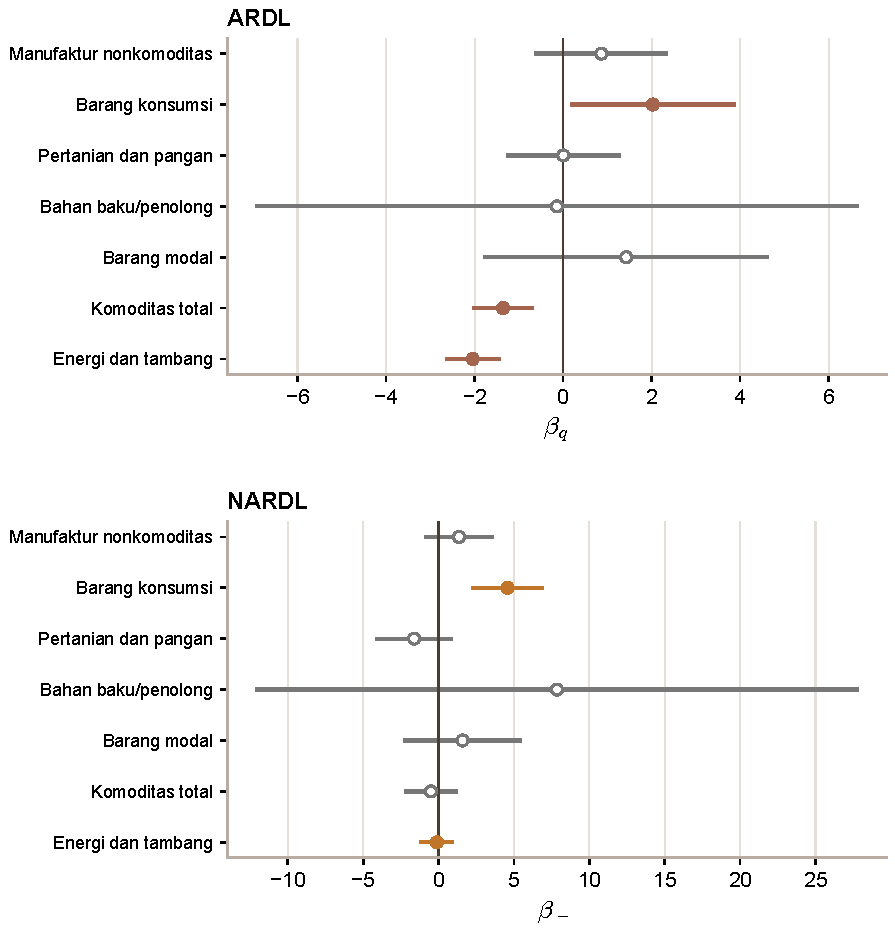
\includegraphics[width=\linewidth,height=.78\textheight,keepaspectratio]{assets/world_goods_forest.pdf}
\caption{Koefisien dan confidence interval tujuh kelompok. Cokelat: lolos pemeriksaan long run dan diagnostic tests. Emas: ada catatan model. Simbol kosong: bukti long run belum cukup.}\label{fig:goodsforest}
\end{figure}

\subsection{Komoditas total dan energi/tambang}
Pada ARDL, koefisien komoditas total sekitar $-1,355$. P-value-nya di bawah 0,001 dan BH sekitar 0,0037. Energi/tambang mempunyai koefisien sekitar $-2,040$ dengan p-value lebih kecil. Keduanya juga lolos pemeriksaan utama.

Dalam model linier ini, rupiah yang melemah berkaitan dengan memburuknya rasio perdagangan kedua kelompok. Hasilnya relevan bagi dugaan bahwa depresiasi tidak selalu memberi perbaikan.

Tetapi penyebabnya belum diketahui. Perubahan bisa berkaitan dengan harga, volume, impor, atau komposisi produk. Energi/tambang juga merupakan bagian komoditas total, sehingga keduanya bukan dua bukti yang sepenuhnya independen.

NARDL belum menguatkan kesimpulan yang sama. Koefisien depresiasi komoditas total sekitar $-0,504$ dan tidak signifikan. Joint-X test belum mendukung walaupun F dan t bounds menolak. Pada energi/tambang, koefisien sekitar $-0,112$ juga tidak signifikan, dengan catatan heteroskedasticity.

Uji asymmetry energi/tambang signifikan, tetapi koefisien depresiasinya tidak. Menguji apakah dua koefisien berbeda tidak sama dengan menguji apakah satu koefisien berbeda dari nol.

\begin{figure}[!htbp]\centering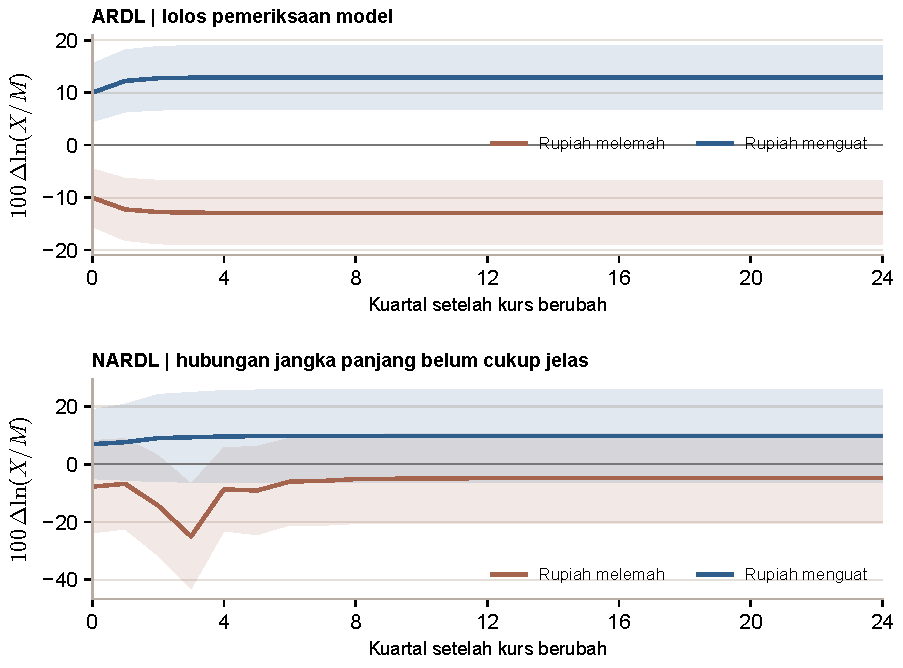
\includegraphics[width=\linewidth]{assets/response_TYPE_WLD_commodity.pdf}
\caption{Komoditas total Indonesia. ARDL mengarah pada pemburukan saat rupiah melemah; NARDL memberi hasil yang lebih tidak pasti.}\label{fig:commodity}
\end{figure}

\subsection{Manufaktur nonkomoditas}
Koefisien ARDL sekitar 0,865 dan koefisien depresiasi NARDL sekitar 1,358. Keduanya belum signifikan pada 5\%, dan pemeriksaan long run belum terpenuhi. Tanda positif belum cukup untuk mengatakan bahwa manufaktur pasti lebih diuntungkan oleh depresiasi.

Tidak signifikan juga belum berarti tidak sensitif. Confidence interval yang lebar bisa mencakup pengaruh yang cukup besar. Untuk menyatakan efek kecil, perlu batas efek yang masuk akal secara ekonomi dan pengujian khusus. Run ini belum melakukannya.

\subsection{Konsumsi, pertanian, bahan baku/penolong, dan modal}
NARDL konsumsi mempunyai koefisien sekitar 4,580 dan signifikan secara nominal maupun BH. Namun ada catatan autocorrelation, heteroskedasticity, RESET, dan CUSUMSQ. Koefisien besar tidak menghilangkan persoalan model ini.

ARDL konsumsi lolos pemeriksaan utama dan garisnya memperlihatkan pola J. Tetapi BH sekitar 0,124, dan confidence interval belum memisahkan kedua fase dengan kuat.

Pada NARDL pertanian/pangan dan modal, F dan t bounds menolak, tetapi joint-X test belum mendukung. Aturan lengkapnya belum terpenuhi. Hasil ini belum dibaca sebagai hubungan long run yang kuat.

Bahan baku/penolong mempunyai confidence interval sangat lebar dan catatan CUSUM. F/t bounds juga belum lengkap. Angka koefisien besar dalam kondisi ini lebih menunjukkan ketidakpastian daripada efek besar yang sudah pasti.

Kelompok bahan baku/penolong hanya menunjukkan penggunaan barang. Ia belum mengukur ketergantungan eksportir pada bahan impor.

\subsection{Contoh hasil yang berbeda menurut mitra}
NARDL pertanian Indonesia--Tiongkok lebih mendukung arah pemburukan. Koefisiennya sekitar $-2,037$, p-value sekitar 0,0016, dan BH sekitar 0,0148. Model juga lolos pemeriksaan utama.

Temuan tersebut berlaku pada rasio perdagangan kelompok ini dengan Tiongkok. Ia belum membuktikan bahwa seluruh ekspor pertanian Indonesia turun akibat depresiasi.

\begin{figure}[!htbp]\centering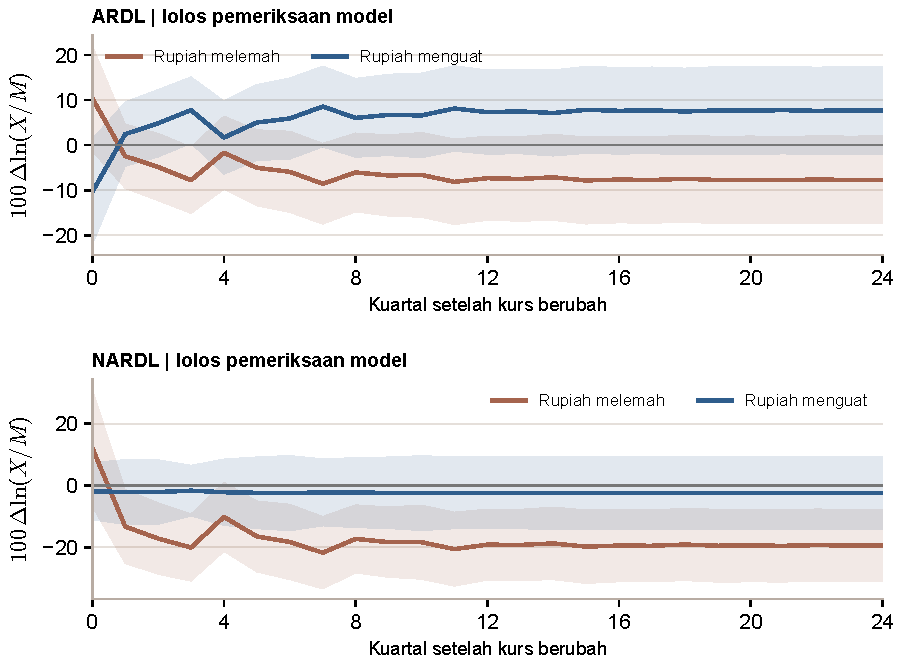
\includegraphics[width=\linewidth]{assets/response_TYPE_CHN_agriculture.pdf}
\caption{Pertanian Indonesia--Tiongkok memberi hasil berbeda dari perdagangan total dengan Tiongkok.}\label{fig:chinaagri}
\end{figure}

Sebaliknya, modal Indonesia--Korea dan konsumsi Indonesia--AS memperlihatkan pola J yang lebih jelas pada confidence interval pointwise. Ada fase awal di bawah nol dan bagian akhir di atas nol. Kedua model lolos pemeriksaan long run dan diagnostic tests.

BH modal Korea sekitar 0,104, sedangkan konsumsi AS sekitar 0,0027. Jadi, kekuatan bukti keduanya tidak persis sama. Pemilihan horizon dan model juga belum tercakup dalam satu uji simultan seluruh jalur.

\begin{figure}[!htbp]\centering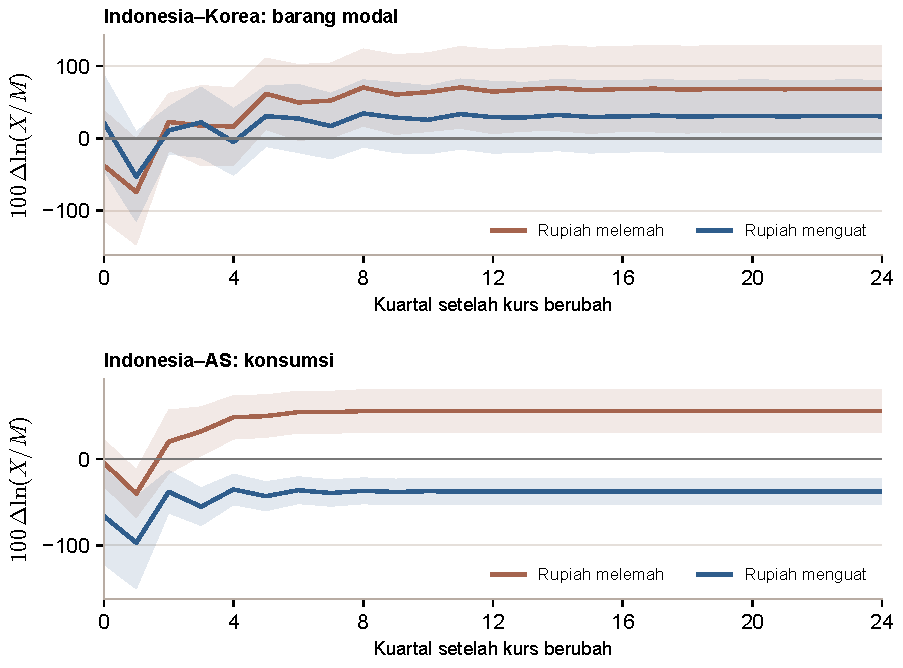
\includegraphics[width=\linewidth]{assets/J_examples.pdf}
\caption{Contoh NARDL dengan fase awal memburuk dan akhir membaik. Confidence interval berlaku per horizon, belum menjadi satu uji seluruh kurva.}\label{fig:Jexamples}
\end{figure}

Secara keseluruhan, hasil tidak memberi satu jawaban untuk semua barang dan pasar. Kita perlu melihat perbedaan tersebut tanpa langsung menyimpulkan bahwa semua komoditas tidak responsif atau selalu dirugikan.

\clearpage\section{Seberapa kuat hasilnya?}\label{sec:diagnostics}
\subsection{Tidak cukup hanya melihat p-value}
Dari 176 model utama, 95 memenuhi keputusan F dan t bounds pada 5\%. Setelah pemeriksaan long run tambahan, jumlahnya menjadi 62. Sebanyak 28 juga lolos diagnostic tests yang dipakai.

Angka 28 tidak berarti hanya 28 model yang benar. Ini hasil dari satu kumpulan aturan pemeriksaan. Kita tetap perlu melihat tes mana yang memberi catatan dan apa artinya bagi kesimpulan.

Diagnostic tests memeriksa residual, yaitu selisih data aktual dengan nilai yang diperkirakan model. Beberapa istilahnya:
\begin{itemize}
\item \textbf{Autocorrelation}: residual masih berkaitan antarperiode.
\item \textbf{Heteroskedasticity dan ARCH}: variasi residual tidak selalu tetap.
\item \textbf{RESET}: ada indikasi bentuk model perlu ditinjau.
\item \textbf{Normality test}: distribusi residual berbeda dari distribusi normal yang diuji.
\item \textbf{CUSUM dan CUSUMSQ}: membantu memeriksa stabilitas sepanjang waktu.
\end{itemize}

Masalah-masalah ini tidak sama. Residual yang tidak normal, misalnya, tidak otomatis berarti OLS tidak konsisten. Menggabungkan semua tes menjadi satu status bersih merupakan pilihan yang cukup hati-hati.

Tes yang tidak menemukan masalah juga belum membuktikan model pasti benar. Sampel kecil bisa membuat tes kurang kuat. Diagnostic tests pun belum menyelesaikan masalah sebab-akibat atau variabel penting yang belum masuk.

\subsection{Bagaimana stabilitas diperiksa?}
CUSUM utama diambil dari Stata \cite{stata}. Nilai jalurnya cocok dengan statistik tersimpan untuk seluruh 176 model utama. Perhitungan independen juga cocok ketika data awal memungkinkan semua parameter dibedakan dengan baik.

Dua pengecualian adalah modal dan konsumsi Australia pada NARDL. Data awalnya belum cukup untuk membedakan semua parameter, atau belum \emph{full rank}. Perhitungan independen menunggu sampai kondisi tersebut terpenuhi, sehingga cara memulainya berbeda dari Stata. Hasil resmi Stata tetap dipakai dan model diberi catatan. Ini berbeda dari model total bilateral Australia.

CUSUMSQ memakai pendekatan Monte Carlo dengan 19.999 simulasi dan seed tetap. Batas pembanding dihitung melalui simulasi yang bisa diulang. Simulasi ini memakai acuan distribusi normal. Hasilnya masih pendekatan, bukan salinan persis tabel paper acuan.

\begin{figure}[!htbp]\centering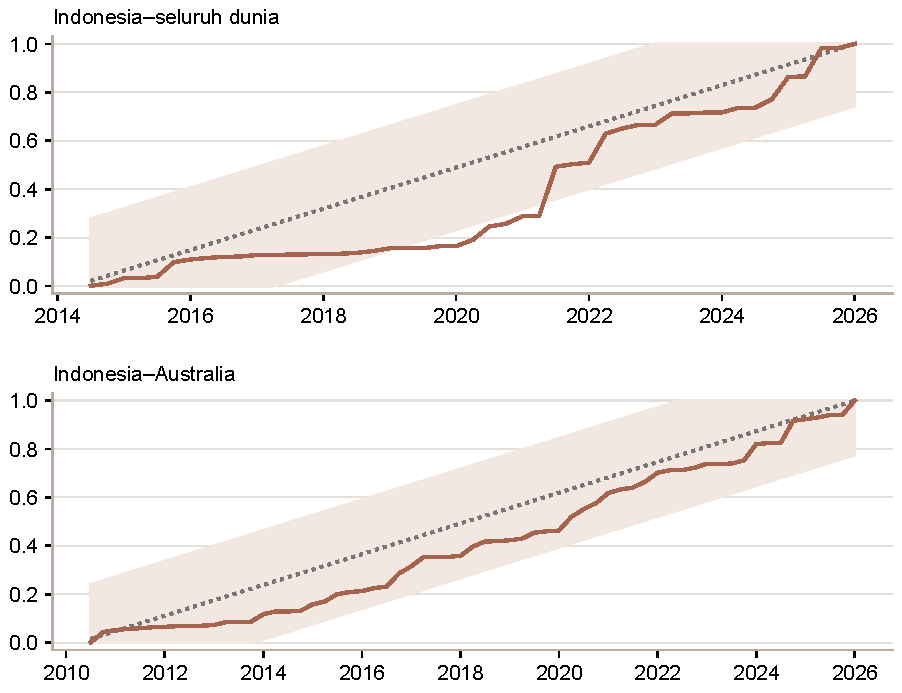
\includegraphics[width=\linewidth]{assets/stability.pdf}
\caption{CUSUMSQ total Indonesia dan Indonesia--Australia. Grafik ini memeriksa stabilitas residual; area berwarna bukan confidence interval efek kurs.}\label{fig:stability}
\end{figure}

Pada total Indonesia, CUSUMSQ memberi catatan stabilitas. Pada Australia, pemeriksaan utama tidak menemukan masalah itu. Perhitungan model juga sudah dicocokkan antara persamaan level dan error correction serta dengan fitted values OLS independen. Cek numerik lulus, tetapi itu belum membuktikan semua asumsi ekonomi benar.

\subsection{Apa itu robustness check?}
Robustness check melihat apakah hasil berubah saat pilihan analisis diubah. Run ini mencoba maksimum lag yang lebih pendek, menambah BCOM, memperpanjang data total ke 2006, memakai WPI India, dan memakai keluarga kurs GEM untuk beberapa mitra.

Arah negatif komoditas total dan energi/tambang bertahan pada beberapa ARDL pembanding. Tetapi sebagian mendapat catatan diagnostic tests. Pada NARDL, koefisien depresiasinya belum signifikan dan status long run dapat berubah menurut lag.

\begin{table}[!htbp]\centering\caption{Robustness checks ARDL komoditas Indonesia}
{\small\setlength{\tabcolsep}{3pt}\renewcommand{\arraystretch}{1.15}
\begin{tabular}{p{0.08\linewidth}p{0.2\linewidth}p{0.08\linewidth}p{0.2\linewidth}p{0.15\linewidth}p{0.12\linewidth}}
\toprule
\textbf{Kel.} & \textbf{Varian} & \textbf{N} & \textbf{Koef. kurs} & \textbf{p} & \textbf{Status}\\
\midrule
G6 & Utama & 61 & -1,355 & \(<0{,}001\) & L+D\\
G6 & Cap 2 & 63 & -1,536 & \(<0{,}001\) & L+D\\
G6 & BCOM & 61 & -1,378 & \(<0{,}001\) & L\\
G7 & Utama & 61 & -2,040 & \(<0{,}001\) & L+D\\
G7 & Cap 2 & 63 & -2,222 & \(<0{,}001\) & L\\
G7 & BCOM & 61 & -2,305 & \(<0{,}001\) & L\\
\bottomrule
\end{tabular}
}\label{tab:sens}
\end{table}

BCOM adalah indeks harga luas. Ia bisa bergerak bersama permintaan global, energi, dan kondisi keuangan. Menambahkannya membantu memeriksa perubahan hasil, tetapi belum membuktikan bahwa harga global adalah penyebab yang sudah berhasil dipisahkan.

Perubahan sumber bisa mengubah konsep dan periode data sekaligus. Jadi, tidak semua robustness check hanya mengubah satu hal pada sampel identik.

Tiga NARDL India dengan BCOM tidak mempunyai hasil bounds finite-sample yang tersedia: komoditas total, energi/tambang, dan bahan baku/penolong. Ketiganya memakai 49 observasi dan 25--27 parameter. Koefisien tetap tersedia; uji yang tidak tersedia tidak diubah menjadi keputusan lolos atau gagal.

\subsection{Mengapa pola J berkurang setelah diperiksa?}
Aturan membaca garis utama di PPT dan paper adalah
\begin{equation}
 \min_{0\le h\le4}R_h^{J,-}<0,\qquad
 \frac{1}{9}\sum_{h=16}^{24}R_h^{J,-}>0.\label{eq:jvisual}
\end{equation}
Artinya, ada setidaknya satu bagian negatif pada tahun pertama dan rata-rata bagian akhir positif. Ini aturan untuk membantu pelaporan, bukan uji J-curve formal paper. Aturan tersebut juga tidak ditetapkan sebelum hasil penelitian dilihat.

\begin{table}[!htbp]\centering\caption{Pola J sebelum dan sesudah pemeriksaan tambahan}
{\small\setlength{\tabcolsep}{3pt}\renewcommand{\arraystretch}{1.15}
\begin{tabular}{p{0.18\linewidth}p{0.12\linewidth}p{0.15\linewidth}p{0.21\linewidth}p{0.23\linewidth}}
\toprule
\textbf{Model} & \textbf{Seri} & \textbf{J titik} & \textbf{J + L+D} & \textbf{Dua fase CI}\\
\midrule
ARDL & 88 & 10 & 1 & 0\\
NARDL & 88 & 24 & 5 & 2\\
\bottomrule
\end{tabular}
}\label{tab:j}
\end{table}

Ada sepuluh pola J pada garis utama ARDL dan 24 pada NARDL. Setelah cek long run dan diagnostic tests, tersisa satu ARDL dan lima NARDL. Jika fase awal dan akhir juga harus terpisah dari nol pada confidence interval yang digunakan, tersisa nol ARDL dan dua NARDL.

Dua NARDL itu adalah modal Korea dan konsumsi AS. Masih ada proses mencari salah satu horizon awal, sehingga hasil ini belum menjadi satu uji simultan semua fase. Kelompok yang tumpang tindih juga membuat jumlah kasus tidak bisa dibaca sebagai frekuensi J-curve pada seluruh perdagangan.

\subsection{Mengapa ARDL dan NARDL bisa berbeda?}
NARDL menambah parameter dan membagi perubahan kurs menjadi dua seri. Seri tersebut juga bisa bergerak bersama aktivitas ekonomi. Pada data terbatas, angka untuk satu arah kurs dapat menjadi lebih tidak pasti.

AIC juga dapat memilih lag berbeda. ARDL yang lebih sederhana bisa lebih presisi, tetapi batasan simetrinya mungkin terlalu kuat. Perbedaan hasil belum otomatis membuktikan salah satunya paling benar.

Karena itu, model tidak dipilih hanya dari tanda yang sesuai hipotesis. Ketidaksepakatan hasil linier dan nonlinear perlu ikut dijelaskan sebagai temuan.

\clearpage\section{Apa kesimpulan yang bisa diambil?}\label{sec:discussion}
\subsection{Depresiasi belum menjadi jaminan perbaikan}
Hasil belum memberi dasar untuk mengatakan bahwa rupiah yang melemah selalu memperbaiki trade balance Indonesia. Model total belum mendukung hubungan long run yang kuat. Setelah dipisah, ada pasar atau kelompok yang mengarah pada perbaikan dan ada yang mengarah pada pemburukan.

Pada ARDL, komoditas total dan energi/tambang memberi hasil yang relevan bagi hipotesis awal. Arah negatifnya bertahan pada beberapa pembanding. Namun NARDL belum menguatkan hasil yang sama, dan sebagian pembanding mempunyai catatan diagnostic tests.

Pangsa komoditas yang besar membuat analisis menurut barang berguna. Tetapi pangsa itu belum membuktikan bahwa harga global menyebabkan koefisien kurs tertentu. Model belum memisahkan harga, volume, impor, dan perubahan komposisi.

\subsection{Tiga kesimpulan yang belum bisa dibuat}
Pertama, hasil rasio belum sama dengan hasil ekspor saja. Ekspor bisa turun tetapi rasio membaik jika impor turun lebih cepat. Ekspor bisa naik sementara rasio memburuk jika impor naik lebih cepat.

Kedua, tidak signifikan belum berarti tidak ada efek. Jika confidence interval lebar, arah dan besarnya justru belum diketahui dengan cukup jelas. Untuk menyatakan efek kecil, perlu batas yang masuk akal secara ekonomi dan pengujian khusus.

Ketiga, signifikan pada satu kelompok dan tidak signifikan pada kelompok lain belum membuktikan bahwa keduanya berbeda secara statistik. Selisih koefisien perlu diuji langsung, dengan memperhatikan periode data dan keterkaitan kelompok.

\subsection{Apa keterbatasan yang paling berpengaruh?}
Versi HS per angka belum diketahui. Mapping yang dipakai menghindari pemaksaan kategori, tetapi belum menghapus masalah perubahan kode dan komposisi.

Periode tiap mitra tidak sama. India lebih pendek, sedangkan AS dan Vietnam berhenti lebih awal. Jadi, perbedaan hasil juga mungkin berkaitan dengan kejadian ekonomi yang berbeda dalam sampelnya.

Perdagangan adalah nilai nominal dan belum disesuaikan musiman. Harga bisa mengubah nilainya meskipun volume tidak banyak berubah. Musiman juga masih perlu diperiksa.

Kurs bisa merespons trade balance atau keduanya merespons kejadian yang sama. Lag belum otomatis memisahkan sebab-akibat. Run ini belum memakai desain kausal yang mengisolasi perubahan kurs dari pengaruh lain.

Banyak model juga diuji. BH membantu membaca sebagian pengujian, tetapi belum mengoreksi seluruh pemilihan model, lag, dan sensitivitas. Menampilkan semua hasil membuat proses transparan, bukan berarti semua risiko pencarian hasil hilang.

\subsection{Apa langkah berikutnya?}
Prioritasnya adalah memperbaiki kesebandingan data dan model. Versi HS perlu diperjelas, hasil pada periode yang sama perlu dibandingkan, dan masalah musiman serta residual perlu ditinjau sesuai diagnostic tests.

Jika fokus akhirnya ekspor, persamaan ekspor terpisah akan lebih langsung menjawabnya. Data kuantitas atau harga yang sesuai juga membantu membedakan perubahan nilai dari volume.

Regresi per kode HS-6 memerlukan cek tambahan. Produk bisa mempunyai nol, perubahan kode, atau data terlalu pendek. Data HS-6 yang tersedia belum berarti semua kode bisa langsung memakai model log yang sama.

\subsection{Ringkasan akhir}
Respons perdagangan Indonesia tidak seragam. Australia dan Malaysia menunjukkan hasil NARDL yang lebih mendukung, tetapi ketahanan signifikansinya berbeda. Komoditas total dan energi/tambang mengarah negatif pada ARDL, namun hasil nonlinear dan robustness checks belum seragam.

Pola J terlihat pada sebagian grafik, tetapi confidence interval dan pemeriksaan model mengurangi jumlah kasus yang lebih kuat. Penelitian belum membuktikan bahwa depresiasi selalu merugikan atau komoditas pasti tidak sensitif terhadap kurs.

Saat membaca, pisahkan angka yang terlihat, seberapa jauh model mendukungnya, dan kemungkinan penjelasan ekonominya. Ini membantu kita memakai temuan tanpa memberi kesimpulan yang lebih kuat daripada datanya.

\clearpage\begin{thebibliography}{99}
\addcontentsline{toc}{section}{Daftar pustaka}
\bibitem{bahmani}
Bahmani-Oskooee, M. dan Fariditavana, H. (2016; terbit daring 2015).
Nonlinear ARDL Approach and the J-Curve Phenomenon.
\emph{Open Economies Review}, 27(1), 51--70.
\url{https://doi.org/10.1007/s11079-015-9369-5}.
Paper lengkap yang diberikan pengguna tersedia pada referensi proyek.

\bibitem{pss}
Pesaran, M. H., Shin, Y. dan Smith, R. J. (2001).
Bounds testing approaches to the analysis of level relationships.
\emph{Journal of Applied Econometrics}, 16(3), 289--326.
\url{https://doi.org/10.1002/jae.616}.

\bibitem{shin}
Shin, Y., Yu, B. dan Greenwood-Nimmo, M. (2014).
Modelling Asymmetric Cointegration and Dynamic Multipliers in a Nonlinear ARDL Framework.
Dalam \emph{Festschrift in Honor of Peter Schmidt}, 281--314.
Springer. \url{https://doi.org/10.1007/978-1-4899-8008-3_9}.

\bibitem{ks}
Kripfganz, S. dan Schneider, D. C. (2023).
ardl: Estimating autoregressive distributed lag and equilibrium correction models.
\emph{The Stata Journal}, 23(4), 983--1019.
\url{https://doi.org/10.1177/1536867X231212434}.

\bibitem{bh}
Benjamini, Y. dan Hochberg, Y. (1995).
Controlling the False Discovery Rate: A Practical and Powerful Approach to Multiple Testing.
\emph{Journal of the Royal Statistical Society: Series B}, 57(1), 289--300.
\url{https://doi.org/10.1111/j.2517-6161.1995.tb02031.x}.

\bibitem{bec}
United Nations Statistics Division (2018).
\emph{Classification by Broad Economic Categories, Revision 5},
ST/ESA/STAT/SER.M/53/Rev.5.
\url{https://unstats.un.org/unsd/trade/classifications/bec.asp}.
Manual dan korespondensi disimpan dalam referensi proyek.

\bibitem{unsdcorr}
United Nations Statistics Division (2022).
\emph{HS--SITC--BEC Correlations dan korespondensi antar revisi HS}.
\url{https://unstats.un.org/unsd/classifications/Econ/}.
File sumber lokal: \texttt{unsd\_correlations\_2022.xlsx}
dan korespondensi HS--SITC dalam folder referensi klasifikasi.

\bibitem{unctad}
UNCTAD (tanpa tahun; salinan lokal diakses 2026).
\emph{SITC Rev.3 Products: Special Groupings Hierarchy},
kelompok komoditas A11.
\url{https://unctadstat.unctad.org/EN/Classifications/DimSitcRev3Products_DsibSpecialGroupings_Hierarchy.pdf}.
Salinan lokal dan manifest unduhan dipertahankan untuk penelusuran.

\bibitem{stata}
StataCorp.
\emph{estat sbcusum: Cumulative sum test for parameter stability}.
Manual resmi Stata.
\url{https://www.stata.com/manuals/tsestatsbcusum.pdf}.

\bibitem{local}
Dokumentasi proyek Tio (2026).
Audit data HS-6, audit validitas makro, manifest sumber dan hasil estimasi.
Berkas lokal pada \path{input/reference/},
\path{output/diagnostics/data/} dan
\path{output/diagnostics/oskooee/}.
Audit cakupan negara pelapor: \path{output/presentation/scope_audit_indonesia.json}.
Statistik dan estimasi naskah menggunakan keluaran run 17 November 2026.
\end{thebibliography}

\clearpage\appendix\section{Cara membaca tabel lengkap}\label{app:read}
Semua 176 model utama dan 340 robustness checks tetap ditampilkan. Ini termasuk hasil yang belum mendukung long run atau mempunyai masalah diagnostic tests.

Koefisien pada ARDL adalah $\beta_q$, sedangkan pada NARDL adalah $\beta_-$. Dengan definisi kurs yang dipakai, positif mengarah pada perbaikan saat depresiasi dan negatif mengarah pada pemburukan. Namun hasil masih perlu memenuhi pemeriksaan model.

\subsection{Kode yang dipakai}
Negara pelapor selalu Indonesia. WLD berarti semua mitra; AUS Australia; CHN Tiongkok; IND India; JPN Jepang; KOR Korea Selatan; MYS Malaysia; SGP Singapura; THA Thailand; USA Amerika Serikat; dan VNM Vietnam.

G0 berarti seluruh barang. G1--G7 mengikuti Tabel~\ref{tab:groups}. Ingat bahwa ketujuh kelompok tidak bisa dijumlahkan menjadi total karena sebagian tumpang tindih.

U berarti model utama dengan maksimum empat lag level. L2 berarti maksimum dua lag. P menambah BCOM. W06 memperpanjang total Indonesia ke 2006+. WPI memakai proksi harga WPI India. FX memakai keluarga kurs GEM. Sebagian perubahan tersebut juga mengubah periode data.

\subsection{Arti status dan p-value}
\textbf{L+D}: pemeriksaan long run dan diagnostic tests yang dipakai terpenuhi. \textbf{L}: long run didukung, tetapi ada catatan diagnostic tests. Tanda \textbf{--}: bukti long run belum cukup atau hasil uji yang diperlukan tidak tersedia.

Status L+D belum berarti koefisien kurs signifikan. Misalnya, model bisa mendukung suatu hubungan long run secara keseluruhan, tetapi angka pengaruh kursnya masih tidak pasti.

Kolom p menunjukkan p-value awal, sedangkan BH menunjukkan hasil koreksi dalam keluarga model utama. BH tidak dihitung untuk model pembanding pada run ini, sehingga kolomnya ditulis --. Angka $<0{,}001$ berarti lebih kecil dari 0,001, bukan nol persis.

N adalah jumlah kuartal yang masuk regresi setelah lag disiapkan. N bukan jumlah bulan atau semua kuartal raw data.

\subsection{Di mana rincian lainnya?}
Workbook \path{output/tables/oskooee/Oskooee_Results.xlsx} memuat koefisien, unit root tests, rentang sampel, dan pemeriksaan model. Rincian lain tersedia dalam \path{results_all_models.csv} dan \path{diagnostic_summary.csv}.

PPT lengkap memuat respons semua 516 model. Paper ini memilih grafik untuk pembahasan, sedangkan tabel berikut tetap mempertahankan semua angka ringkasnya.

\clearpage\section{Semua 176 model utama}
\noindent Semua perdagangan adalah milik Indonesia. WLD berarti seluruh mitra. Kode dan status dijelaskan pada Lampiran~\ref{app:read}. Angka tabel sama dengan paper versi sebelumnya.
{\footnotesize\setlength{\tabcolsep}{3pt}\renewcommand{\arraystretch}{1.15}
\begin{longtable}{p{0.075\linewidth}p{0.05\linewidth}p{0.09\linewidth}p{0.04\linewidth}p{0.05\linewidth}p{0.1\linewidth}p{0.085\linewidth}p{0.085\linewidth}p{0.075\linewidth}}
\toprule
\textbf{Mitra} & \textbf{Kel.} & \textbf{Model} & \textbf{N} & \textbf{Var.} & \textbf{Koef.} & \textbf{p} & \textbf{BH} & \textbf{Status}\\
\midrule
\endfirsthead
\toprule
\textbf{Mitra} & \textbf{Kel.} & \textbf{Model} & \textbf{N} & \textbf{Var.} & \textbf{Koef.} & \textbf{p} & \textbf{BH} & \textbf{Status}\\
\midrule
\endhead
\midrule\multicolumn{9}{r}{\footnotesize Bersambung ke halaman berikutnya}\\\endfoot
\bottomrule\endlastfoot
AUS & G3 & ARDL & 77 & U & -1,770 & 0,043 & 0,165 & --\\
AUS & G3 & NARDL & 77 & U & -3,345 & \(<0{,}001\) & 0,004 & L\\
AUS & G5 & ARDL & 77 & U & 4,002 & 0,120 & 0,307 & --\\
AUS & G5 & NARDL & 77 & U & 7,466 & 0,041 & 0,138 & --\\
AUS & G6 & ARDL & 77 & U & 1,701 & 0,008 & 0,103 & L+D\\
AUS & G6 & NARDL & 77 & U & 1,379 & 0,142 & 0,332 & L+D\\
AUS & G2 & ARDL & 77 & U & 0,704 & 0,316 & 0,544 & --\\
AUS & G2 & NARDL & 77 & U & 1,088 & 0,285 & 0,488 & --\\
AUS & G7 & ARDL & 77 & U & 3,265 & 0,026 & 0,121 & L\\
AUS & G7 & NARDL & 77 & U & 5,725 & 0,006 & 0,036 & L\\
AUS & G4 & ARDL & 77 & U & 1,608 & 0,024 & 0,121 & L\\
AUS & G4 & NARDL & 77 & U & 2,518 & 0,010 & 0,053 & L+D\\
AUS & G1 & ARDL & 77 & U & 0,919 & 0,460 & 0,656 & --\\
AUS & G1 & NARDL & 77 & U & 5,628 & 0,003 & 0,023 & --\\
AUS & G0 & ARDL & 77 & U & 2,084 & 0,002 & 0,021 & L+D\\
AUS & G0 & NARDL & 77 & U & 3,356 & \(<0{,}001\) & 0,004 & L+D\\
CHN & G3 & ARDL & 78 & U & -0,809 & 0,119 & 0,307 & L+D\\
CHN & G3 & NARDL & 78 & U & -2,036 & 0,002 & 0,015 & L+D\\
CHN & G5 & ARDL & 78 & U & 1,211 & 0,325 & 0,544 & L\\
CHN & G5 & NARDL & 78 & U & 0,595 & 0,764 & 0,842 & L\\
CHN & G6 & ARDL & 78 & U & -2,216 & 0,005 & 0,103 & L\\
CHN & G6 & NARDL & 78 & U & -3,458 & \(<0{,}001\) & 0,003 & L\\
CHN & G2 & ARDL & 78 & U & -0,569 & 0,567 & 0,752 & --\\
CHN & G2 & NARDL & 78 & U & -2,711 & 0,031 & 0,108 & L+D\\
CHN & G7 & ARDL & 78 & U & -1,924 & 0,101 & 0,300 & --\\
CHN & G7 & NARDL & 78 & U & -3,658 & 0,022 & 0,101 & L\\
CHN & G4 & ARDL & 78 & U & -3,291 & 0,046 & 0,168 & --\\
CHN & G4 & NARDL & 78 & U & -6,234 & 0,004 & 0,023 & --\\
CHN & G1 & ARDL & 78 & U & 0,300 & 0,878 & 0,955 & --\\
CHN & G1 & NARDL & 78 & U & 3,033 & 0,663 & 0,763 & --\\
CHN & G0 & ARDL & 78 & U & -1,886 & 0,059 & 0,148 & --\\
CHN & G0 & NARDL & 78 & U & -2,727 & 0,250 & 0,350 & --\\
IND & G3 & ARDL & 49 & U & 6,325 & 0,645 & 0,823 & --\\
IND & G3 & NARDL & 49 & U & -5,076 & 0,316 & 0,503 & L\\
IND & G5 & ARDL & 49 & U & 1,012 & 0,913 & 0,963 & --\\
IND & G5 & NARDL & 49 & U & 0,815 & 0,939 & 0,970 & --\\
IND & G6 & ARDL & 49 & U & 5,476 & 0,549 & 0,742 & --\\
IND & G6 & NARDL & 49 & U & -4,569 & 0,320 & 0,503 & L+D\\
IND & G2 & ARDL & 49 & U & 3,982 & 0,535 & 0,736 & --\\
IND & G2 & NARDL & 49 & U & -8,904 & 0,090 & 0,263 & L\\
IND & G7 & ARDL & 49 & U & 7,828 & 0,358 & 0,574 & --\\
IND & G7 & NARDL & 49 & U & -4,506 & 0,346 & 0,526 & L+D\\
IND & G4 & ARDL & 49 & U & 10,846 & 0,240 & 0,463 & --\\
IND & G4 & NARDL & 49 & U & 2,938 & 0,702 & 0,795 & --\\
IND & G1 & ARDL & 49 & U & -4,502 & 0,393 & 0,606 & --\\
IND & G1 & NARDL & 49 & U & -6,379 & 0,179 & 0,377 & --\\
IND & G0 & ARDL & 49 & U & 5,254 & 0,437 & 0,486 & --\\
IND & G0 & NARDL & 49 & U & -6,443 & 0,236 & 0,350 & --\\
JPN & G3 & ARDL & 78 & U & -0,075 & 0,925 & 0,963 & --\\
JPN & G3 & NARDL & 78 & U & -1,712 & 0,009 & 0,047 & --\\
JPN & G5 & ARDL & 78 & U & -3,068 & 0,075 & 0,241 & --\\
JPN & G5 & NARDL & 78 & U & -4,687 & 0,002 & 0,018 & --\\
JPN & G6 & ARDL & 78 & U & -1,771 & 0,009 & 0,103 & L\\
JPN & G6 & NARDL & 78 & U & -0,710 & 0,493 & 0,612 & L+D\\
JPN & G2 & ARDL & 78 & U & -0,718 & 0,337 & 0,553 & L\\
JPN & G2 & NARDL & 78 & U & -1,246 & 0,244 & 0,448 & L\\
JPN & G7 & ARDL & 78 & U & -2,107 & 0,016 & 0,119 & L\\
JPN & G7 & NARDL & 78 & U & -0,160 & 0,894 & 0,945 & L+D\\
JPN & G4 & ARDL & 78 & U & -2,347 & 0,021 & 0,121 & --\\
JPN & G4 & NARDL & 78 & U & -3,048 & 0,002 & 0,015 & --\\
JPN & G1 & ARDL & 78 & U & -1,171 & 0,166 & 0,375 & --\\
JPN & G1 & NARDL & 78 & U & -1,477 & 0,159 & 0,350 & --\\
JPN & G0 & ARDL & 78 & U & -2,106 & 0,017 & 0,058 & --\\
JPN & G0 & NARDL & 78 & U & -2,456 & 0,006 & 0,020 & --\\
KOR & G3 & ARDL & 78 & U & 1,449 & 0,056 & 0,187 & --\\
KOR & G3 & NARDL & 78 & U & 1,601 & 0,241 & 0,448 & --\\
KOR & G5 & ARDL & 78 & U & 1,416 & 0,420 & 0,622 & --\\
KOR & G5 & NARDL & 78 & U & 7,147 & 0,027 & 0,104 & L+D\\
KOR & G6 & ARDL & 78 & U & -0,370 & 0,857 & 0,955 & --\\
KOR & G6 & NARDL & 78 & U & 4,662 & 0,092 & 0,263 & --\\
KOR & G2 & ARDL & 78 & U & 7,941 & 0,118 & 0,307 & --\\
KOR & G2 & NARDL & 78 & U & 0,875 & 0,945 & 0,970 & --\\
KOR & G7 & ARDL & 78 & U & -0,712 & 0,773 & 0,910 & --\\
KOR & G7 & NARDL & 78 & U & 5,815 & 0,109 & 0,279 & --\\
KOR & G4 & ARDL & 78 & U & 0,887 & 0,652 & 0,823 & --\\
KOR & G4 & NARDL & 78 & U & 10,950 & 0,102 & 0,275 & --\\
KOR & G1 & ARDL & 78 & U & 1,747 & 0,055 & 0,187 & --\\
KOR & G1 & NARDL & 78 & U & 4,717 & 0,001 & 0,013 & --\\
KOR & G0 & ARDL & 78 & U & -0,074 & 0,944 & 0,944 & --\\
KOR & G0 & NARDL & 78 & U & 3,935 & 0,144 & 0,288 & --\\
MYS & G3 & ARDL & 78 & U & 0,338 & 0,803 & 0,922 & --\\
MYS & G3 & NARDL & 78 & U & 3,464 & 0,181 & 0,377 & --\\
MYS & G5 & ARDL & 78 & U & 0,178 & 0,751 & 0,904 & L+D\\
MYS & G5 & NARDL & 78 & U & 0,784 & 0,468 & 0,610 & L+D\\
MYS & G6 & ARDL & 78 & U & -1,290 & 0,088 & 0,270 & L+D\\
MYS & G6 & NARDL & 78 & U & 1,444 & 0,258 & 0,461 & L+D\\
MYS & G2 & ARDL & 78 & U & -0,746 & 0,695 & 0,850 & --\\
MYS & G2 & NARDL & 78 & U & 4,491 & 0,068 & 0,219 & --\\
MYS & G7 & ARDL & 78 & U & -1,376 & 0,116 & 0,307 & L+D\\
MYS & G7 & NARDL & 78 & U & 1,117 & 0,483 & 0,610 & L+D\\
MYS & G4 & ARDL & 78 & U & -0,645 & 0,408 & 0,617 & --\\
MYS & G4 & NARDL & 78 & U & 1,176 & 0,309 & 0,503 & --\\
MYS & G1 & ARDL & 78 & U & 0,285 & 0,845 & 0,955 & --\\
MYS & G1 & NARDL & 78 & U & 1,939 & 0,406 & 0,578 & --\\
MYS & G0 & ARDL & 78 & U & -0,716 & 0,081 & 0,163 & L\\
MYS & G0 & NARDL & 78 & U & 1,346 & 0,024 & 0,059 & L+D\\
SGP & G3 & ARDL & 78 & U & 5,982 & 0,027 & 0,121 & --\\
SGP & G3 & NARDL & 78 & U & 4,941 & 0,092 & 0,263 & --\\
SGP & G5 & ARDL & 78 & U & -0,469 & 0,669 & 0,831 & --\\
SGP & G5 & NARDL & 78 & U & -1,303 & 0,470 & 0,610 & --\\
SGP & G6 & ARDL & 78 & U & -1,192 & 0,025 & 0,121 & --\\
SGP & G6 & NARDL & 78 & U & -0,701 & 0,483 & 0,610 & --\\
SGP & G2 & ARDL & 78 & U & 2,616 & 0,325 & 0,544 & L\\
SGP & G2 & NARDL & 78 & U & -0,102 & 0,985 & 0,991 & --\\
SGP & G7 & ARDL & 78 & U & -1,383 & 0,016 & 0,119 & --\\
SGP & G7 & NARDL & 78 & U & -0,709 & 0,504 & 0,617 & --\\
SGP & G4 & ARDL & 78 & U & 0,424 & 0,604 & 0,788 & --\\
SGP & G4 & NARDL & 78 & U & -2,032 & 0,022 & 0,101 & L\\
SGP & G1 & ARDL & 78 & U & 0,007 & 0,994 & 0,994 & --\\
SGP & G1 & NARDL & 78 & U & -1,544 & 0,308 & 0,503 & --\\
SGP & G0 & ARDL & 78 & U & -0,451 & 0,432 & 0,486 & --\\
SGP & G0 & NARDL & 78 & U & -0,262 & 0,810 & 0,810 & --\\
THA & G3 & ARDL & 78 & U & 1,906 & 0,216 & 0,442 & --\\
THA & G3 & NARDL & 78 & U & 3,848 & 0,155 & 0,350 & L\\
THA & G5 & ARDL & 78 & U & -1,027 & 0,433 & 0,629 & --\\
THA & G5 & NARDL & 78 & U & 2,593 & 0,355 & 0,526 & --\\
THA & G6 & ARDL & 78 & U & 1,047 & 0,137 & 0,341 & --\\
THA & G6 & NARDL & 78 & U & 3,454 & 0,024 & 0,104 & --\\
THA & G2 & ARDL & 78 & U & 2,543 & 0,015 & 0,119 & L\\
THA & G2 & NARDL & 78 & U & 0,354 & 0,896 & 0,945 & --\\
THA & G7 & ARDL & 78 & U & -0,592 & 0,270 & 0,496 & --\\
THA & G7 & NARDL & 78 & U & 0,755 & 0,594 & 0,703 & --\\
THA & G4 & ARDL & 78 & U & 1,063 & 0,031 & 0,124 & L+D\\
THA & G4 & NARDL & 78 & U & -1,568 & 0,124 & 0,309 & L+D\\
THA & G1 & ARDL & 78 & U & 1,001 & 0,218 & 0,442 & --\\
THA & G1 & NARDL & 78 & U & 0,564 & 0,766 & 0,842 & --\\
THA & G0 & ARDL & 78 & U & 1,180 & 0,006 & 0,031 & L\\
THA & G0 & NARDL & 78 & U & 0,950 & 0,280 & 0,350 & L\\
USA & G3 & ARDL & 75 & U & -0,836 & 0,017 & 0,119 & L+D\\
USA & G3 & NARDL & 75 & U & 0,622 & 0,278 & 0,487 & L+D\\
USA & G5 & ARDL & 75 & U & 1,166 & 0,780 & 0,910 & --\\
USA & G5 & NARDL & 75 & U & 4,530 & 0,434 & 0,587 & --\\
USA & G6 & ARDL & 75 & U & -0,088 & 0,912 & 0,963 & --\\
USA & G6 & NARDL & 75 & U & 3,592 & \(<0{,}001\) & 0,008 & L\\
USA & G2 & ARDL & 75 & U & -0,335 & 0,880 & 0,955 & --\\
USA & G2 & NARDL & 75 & U & 5,861 & \(<0{,}001\) & 0,003 & L+D\\
USA & G7 & ARDL & 75 & U & 5,869 & 0,214 & 0,442 & --\\
USA & G7 & NARDL & 75 & U & 13,527 & 0,354 & 0,526 & --\\
USA & G4 & ARDL & 75 & U & -0,313 & 0,517 & 0,723 & L\\
USA & G4 & NARDL & 75 & U & 2,924 & \(<0{,}001\) & 0,010 & L\\
USA & G1 & ARDL & 75 & U & 1,517 & 0,196 & 0,430 & --\\
USA & G1 & NARDL & 75 & U & 2,189 & 0,142 & 0,332 & --\\
USA & G0 & ARDL & 75 & U & 0,989 & 0,163 & 0,272 & --\\
USA & G0 & NARDL & 75 & U & 3,095 & 0,006 & 0,020 & --\\
VNM & G3 & ARDL & 74 & U & 5,911 & 0,009 & 0,103 & --\\
VNM & G3 & NARDL & 74 & U & 7,260 & 0,026 & 0,104 & --\\
VNM & G5 & ARDL & 74 & U & 2,773 & 0,148 & 0,356 & --\\
VNM & G5 & NARDL & 74 & U & -0,961 & 0,621 & 0,725 & L\\
VNM & G6 & ARDL & 74 & U & 2,123 & 0,252 & 0,474 & --\\
VNM & G6 & NARDL & 74 & U & 2,287 & 0,429 & 0,587 & --\\
VNM & G2 & ARDL & 74 & U & 3,995 & 0,006 & 0,103 & L\\
VNM & G2 & NARDL & 74 & U & 4,684 & 0,031 & 0,108 & L\\
VNM & G7 & ARDL & 74 & U & -3,966 & 0,019 & 0,121 & L\\
VNM & G7 & NARDL & 74 & U & -4,206 & 0,103 & 0,275 & L\\
VNM & G4 & ARDL & 74 & U & -1,282 & 0,158 & 0,368 & L\\
VNM & G4 & NARDL & 74 & U & -2,069 & 0,186 & 0,377 & L\\
VNM & G1 & ARDL & 74 & U & 2,785 & 0,300 & 0,536 & --\\
VNM & G1 & NARDL & 74 & U & -0,025 & 0,991 & 0,991 & --\\
VNM & G0 & ARDL & 74 & U & 1,389 & 0,205 & 0,293 & --\\
VNM & G0 & NARDL & 74 & U & -0,551 & 0,737 & 0,810 & --\\
WLD & G3 & ARDL & 61 & U & 0,005 & 0,993 & 0,994 & --\\
WLD & G3 & NARDL & 61 & U & -1,621 & 0,192 & 0,380 & --\\
WLD & G5 & ARDL & 61 & U & 1,425 & 0,373 & 0,586 & --\\
WLD & G5 & NARDL & 61 & U & 1,589 & 0,402 & 0,578 & --\\
WLD & G6 & ARDL & 61 & U & -1,355 & \(<0{,}001\) & 0,004 & L+D\\
WLD & G6 & NARDL & 61 & U & -0,504 & 0,539 & 0,649 & --\\
WLD & G2 & ARDL & 61 & U & 2,026 & 0,031 & 0,124 & L+D\\
WLD & G2 & NARDL & 61 & U & 4,580 & \(<0{,}001\) & 0,004 & L\\
WLD & G7 & ARDL & 61 & U & -2,040 & \(<0{,}001\) & \(<0{,}001\) & L+D\\
WLD & G7 & NARDL & 61 & U & -0,112 & 0,827 & 0,897 & L\\
WLD & G4 & ARDL & 61 & U & -0,139 & 0,967 & 0,993 & --\\
WLD & G4 & NARDL & 61 & U & 7,851 & 0,431 & 0,587 & --\\
WLD & G1 & ARDL & 61 & U & 0,865 & 0,241 & 0,463 & --\\
WLD & G1 & NARDL & 61 & U & 1,358 & 0,218 & 0,420 & --\\
WLD & G0 & ARDL & 61 & U & 0,429 & 0,661 & 0,661 & --\\
WLD & G0 & NARDL & 61 & U & 2,572 & 0,040 & 0,040 & --\\
\end{longtable}
}

\clearpage\section{Semua 340 robustness checks}
\noindent Periode model pembanding bisa berbeda. BH tidak dihitung untuk keluarga model pembanding pada run ini.
{\footnotesize\setlength{\tabcolsep}{3pt}\renewcommand{\arraystretch}{1.15}
\begin{longtable}{p{0.075\linewidth}p{0.05\linewidth}p{0.09\linewidth}p{0.04\linewidth}p{0.05\linewidth}p{0.1\linewidth}p{0.085\linewidth}p{0.085\linewidth}p{0.075\linewidth}}
\toprule
\textbf{Mitra} & \textbf{Kel.} & \textbf{Model} & \textbf{N} & \textbf{Var.} & \textbf{Koef.} & \textbf{p} & \textbf{BH} & \textbf{Status}\\
\midrule
\endfirsthead
\toprule
\textbf{Mitra} & \textbf{Kel.} & \textbf{Model} & \textbf{N} & \textbf{Var.} & \textbf{Koef.} & \textbf{p} & \textbf{BH} & \textbf{Status}\\
\midrule
\endhead
\midrule\multicolumn{9}{r}{\footnotesize Bersambung ke halaman berikutnya}\\\endfoot
\bottomrule\endlastfoot
AUS & G3 & ARDL & 77 & P & -1,803 & 0,153 & -- & --\\
AUS & G3 & NARDL & 77 & P & -3,639 & \(<0{,}001\) & -- & L\\
AUS & G5 & ARDL & 77 & P & 3,972 & 0,266 & -- & --\\
AUS & G5 & NARDL & 77 & P & 6,788 & 0,094 & -- & --\\
AUS & G6 & ARDL & 77 & P & -0,374 & 0,678 & -- & L+D\\
AUS & G6 & NARDL & 77 & P & -0,914 & 0,313 & -- & L\\
AUS & G2 & ARDL & 77 & P & 1,244 & 0,189 & -- & --\\
AUS & G2 & NARDL & 77 & P & 1,141 & 0,292 & -- & --\\
AUS & G7 & ARDL & 77 & P & 2,080 & 0,195 & -- & L+D\\
AUS & G7 & NARDL & 77 & P & 4,137 & 0,022 & -- & L+D\\
AUS & G4 & ARDL & 77 & P & 0,996 & 0,267 & -- & L\\
AUS & G4 & NARDL & 77 & P & 1,618 & 0,122 & -- & L+D\\
AUS & G1 & ARDL & 77 & P & 0,919 & 0,603 & -- & --\\
AUS & G1 & NARDL & 77 & P & 4,610 & 0,029 & -- & --\\
CHN & G3 & ARDL & 78 & P & -0,171 & 0,641 & -- & L+D\\
CHN & G3 & NARDL & 78 & P & -1,336 & 0,020 & -- & L+D\\
CHN & G5 & ARDL & 78 & P & 0,970 & 0,457 & -- & --\\
CHN & G5 & NARDL & 78 & P & -1,667 & 0,418 & -- & L\\
CHN & G6 & ARDL & 78 & P & -1,437 & 0,049 & -- & L\\
CHN & G6 & NARDL & 78 & P & -2,840 & 0,032 & -- & L\\
CHN & G2 & ARDL & 78 & P & 0,211 & 0,844 & -- & --\\
CHN & G2 & NARDL & 78 & P & -2,343 & 0,133 & -- & L+D\\
CHN & G7 & ARDL & 78 & P & -1,692 & 0,204 & -- & --\\
CHN & G7 & NARDL & 78 & P & -3,921 & 0,128 & -- & --\\
CHN & G4 & ARDL & 78 & P & -10,879 & 0,671 & -- & --\\
CHN & G4 & NARDL & 78 & P & -5,276 & 0,069 & -- & --\\
CHN & G1 & ARDL & 78 & P & -0,619 & 0,751 & -- & --\\
CHN & G1 & NARDL & 78 & P & 3,392 & 0,634 & -- & --\\
IND & G3 & ARDL & 49 & P & 5,989 & 0,336 & -- & --\\
IND & G3 & NARDL & 49 & P & 2,367 & 0,708 & -- & --\\
IND & G5 & ARDL & 49 & P & 4,031 & 0,602 & -- & --\\
IND & G5 & NARDL & 49 & P & 4,253 & 0,661 & -- & --\\
IND & G6 & ARDL & 49 & P & 4,372 & 0,086 & -- & L+D\\
IND & G6 & NARDL & 49 & P & -2,073 & 0,506 & -- & --\\
IND & G2 & ARDL & 49 & P & 3,604 & 0,334 & -- & --\\
IND & G2 & NARDL & 49 & P & -4,509 & 0,192 & -- & L\\
IND & G7 & ARDL & 49 & P & 5,995 & 0,303 & -- & --\\
IND & G7 & NARDL & 49 & P & -7,181 & 0,023 & -- & --\\
IND & G4 & ARDL & 49 & P & 15,059 & 0,435 & -- & --\\
IND & G4 & NARDL & 49 & P & 12,149 & 0,614 & -- & --\\
IND & G1 & ARDL & 49 & P & 0,272 & 0,895 & -- & --\\
IND & G1 & NARDL & 49 & P & 0,215 & 0,929 & -- & --\\
JPN & G3 & ARDL & 78 & P & -0,536 & 0,613 & -- & --\\
JPN & G3 & NARDL & 78 & P & -1,996 & 0,026 & -- & --\\
JPN & G5 & ARDL & 78 & P & -3,468 & 0,188 & -- & --\\
JPN & G5 & NARDL & 78 & P & -6,547 & 0,003 & -- & --\\
JPN & G6 & ARDL & 78 & P & -1,534 & 0,025 & -- & L+D\\
JPN & G6 & NARDL & 78 & P & 0,226 & 0,846 & -- & L+D\\
JPN & G2 & ARDL & 78 & P & -0,659 & 0,379 & -- & L\\
JPN & G2 & NARDL & 78 & P & -0,452 & 0,706 & -- & L\\
JPN & G7 & ARDL & 78 & P & -2,007 & 0,022 & -- & L\\
JPN & G7 & NARDL & 78 & P & 0,771 & 0,588 & -- & L+D\\
JPN & G4 & ARDL & 78 & P & -2,522 & 0,037 & -- & --\\
JPN & G4 & NARDL & 78 & P & -2,930 & 0,057 & -- & --\\
JPN & G1 & ARDL & 78 & P & -2,257 & 0,055 & -- & --\\
JPN & G1 & NARDL & 78 & P & -2,745 & 0,034 & -- & --\\
KOR & G3 & ARDL & 78 & P & 1,390 & \(<0{,}001\) & -- & L\\
KOR & G3 & NARDL & 78 & P & 2,348 & \(<0{,}001\) & -- & L\\
KOR & G5 & ARDL & 78 & P & 1,397 & 0,444 & -- & --\\
KOR & G5 & NARDL & 78 & P & 7,249 & 0,019 & -- & --\\
KOR & G6 & ARDL & 78 & P & -0,718 & 0,775 & -- & --\\
KOR & G6 & NARDL & 78 & P & 5,197 & 0,280 & -- & --\\
KOR & G2 & ARDL & 78 & P & 8,328 & 0,078 & -- & --\\
KOR & G2 & NARDL & 78 & P & 2,899 & 0,795 & -- & --\\
KOR & G7 & ARDL & 78 & P & -1,169 & 0,727 & -- & --\\
KOR & G7 & NARDL & 78 & P & 6,791 & 0,302 & -- & --\\
KOR & G4 & ARDL & 78 & P & 0,809 & 0,607 & -- & --\\
KOR & G4 & NARDL & 78 & P & 14,466 & 0,174 & -- & --\\
KOR & G1 & ARDL & 78 & P & 1,704 & 0,074 & -- & --\\
KOR & G1 & NARDL & 78 & P & 4,733 & 0,002 & -- & --\\
MYS & G3 & ARDL & 78 & P & -0,389 & 0,746 & -- & --\\
MYS & G3 & NARDL & 78 & P & 2,669 & 0,120 & -- & --\\
MYS & G5 & ARDL & 78 & P & 0,103 & 0,834 & -- & L+D\\
MYS & G5 & NARDL & 78 & P & 0,341 & 0,736 & -- & L+D\\
MYS & G6 & ARDL & 78 & P & -0,701 & 0,378 & -- & --\\
MYS & G6 & NARDL & 78 & P & 1,152 & 0,371 & -- & L+D\\
MYS & G2 & ARDL & 78 & P & 1,383 & 0,641 & -- & --\\
MYS & G2 & NARDL & 78 & P & 6,257 & 0,011 & -- & --\\
MYS & G7 & ARDL & 78 & P & -0,811 & 0,315 & -- & L+D\\
MYS & G7 & NARDL & 78 & P & 0,462 & 0,760 & -- & L+D\\
MYS & G4 & ARDL & 78 & P & -0,523 & 0,411 & -- & --\\
MYS & G4 & NARDL & 78 & P & 1,546 & 0,069 & -- & L\\
MYS & G1 & ARDL & 78 & P & 0,149 & 0,909 & -- & --\\
MYS & G1 & NARDL & 78 & P & 1,128 & 0,624 & -- & --\\
SGP & G3 & ARDL & 78 & P & 6,741 & 0,082 & -- & --\\
SGP & G3 & NARDL & 78 & P & 4,384 & 0,138 & -- & --\\
SGP & G5 & ARDL & 78 & P & -0,663 & 0,562 & -- & --\\
SGP & G5 & NARDL & 78 & P & 0,366 & 0,884 & -- & --\\
SGP & G6 & ARDL & 78 & P & -0,766 & 0,097 & -- & L\\
SGP & G6 & NARDL & 78 & P & -0,210 & 0,817 & -- & L\\
SGP & G2 & ARDL & 78 & P & 2,333 & 0,410 & -- & --\\
SGP & G2 & NARDL & 78 & P & -0,273 & 0,961 & -- & --\\
SGP & G7 & ARDL & 78 & P & -0,268 & 0,662 & -- & L\\
SGP & G7 & NARDL & 78 & P & -0,033 & 0,969 & -- & L\\
SGP & G4 & ARDL & 78 & P & 0,219 & 0,794 & -- & --\\
SGP & G4 & NARDL & 78 & P & -2,065 & 0,022 & -- & L\\
SGP & G1 & ARDL & 78 & P & -0,293 & 0,780 & -- & --\\
SGP & G1 & NARDL & 78 & P & 0,500 & 0,792 & -- & --\\
THA & G3 & ARDL & 78 & P & 1,864 & 0,139 & -- & L\\
THA & G3 & NARDL & 78 & P & 5,228 & 0,035 & -- & L\\
THA & G5 & ARDL & 78 & P & -1,181 & 0,303 & -- & --\\
THA & G5 & NARDL & 78 & P & 1,999 & 0,413 & -- & L\\
THA & G6 & ARDL & 78 & P & 1,262 & 0,101 & -- & --\\
THA & G6 & NARDL & 78 & P & 3,030 & 0,050 & -- & --\\
THA & G2 & ARDL & 78 & P & 2,405 & 0,013 & -- & L\\
THA & G2 & NARDL & 78 & P & 0,087 & 0,965 & -- & L\\
THA & G7 & ARDL & 78 & P & -0,811 & 0,142 & -- & --\\
THA & G7 & NARDL & 78 & P & -0,378 & 0,739 & -- & --\\
THA & G4 & ARDL & 78 & P & 0,860 & 0,100 & -- & L+D\\
THA & G4 & NARDL & 78 & P & -0,961 & 0,375 & -- & L\\
THA & G1 & ARDL & 78 & P & 0,883 & 0,284 & -- & --\\
THA & G1 & NARDL & 78 & P & 0,555 & 0,733 & -- & --\\
USA & G3 & ARDL & 75 & P & -0,784 & 0,049 & -- & L+D\\
USA & G3 & NARDL & 75 & P & 0,594 & 0,308 & -- & L\\
USA & G5 & ARDL & 75 & P & 0,392 & 0,910 & -- & --\\
USA & G5 & NARDL & 75 & P & 0,258 & 0,961 & -- & --\\
USA & G6 & ARDL & 75 & P & 1,215 & 0,472 & -- & --\\
USA & G6 & NARDL & 75 & P & 3,305 & \(<0{,}001\) & -- & L+D\\
USA & G2 & ARDL & 75 & P & 0,502 & 0,857 & -- & --\\
USA & G2 & NARDL & 75 & P & 5,114 & \(<0{,}001\) & -- & L+D\\
USA & G7 & ARDL & 75 & P & 10,099 & 0,146 & -- & --\\
USA & G7 & NARDL & 75 & P & 11,962 & 0,027 & -- & --\\
USA & G4 & ARDL & 75 & P & 1,918 & 0,168 & -- & --\\
USA & G4 & NARDL & 75 & P & 3,063 & \(<0{,}001\) & -- & L\\
USA & G1 & ARDL & 75 & P & 0,384 & 0,705 & -- & --\\
USA & G1 & NARDL & 75 & P & 0,643 & 0,699 & -- & --\\
VNM & G3 & ARDL & 74 & P & 6,934 & 0,001 & -- & L+D\\
VNM & G3 & NARDL & 74 & P & 8,952 & 0,002 & -- & L\\
VNM & G5 & ARDL & 74 & P & 3,639 & 0,132 & -- & --\\
VNM & G5 & NARDL & 74 & P & -1,052 & 0,640 & -- & L\\
VNM & G6 & ARDL & 74 & P & 3,707 & 0,048 & -- & L\\
VNM & G6 & NARDL & 74 & P & 4,373 & 0,110 & -- & L\\
VNM & G2 & ARDL & 74 & P & 4,466 & 0,001 & -- & L\\
VNM & G2 & NARDL & 74 & P & 3,771 & 0,032 & -- & L\\
VNM & G7 & ARDL & 74 & P & -4,044 & 0,033 & -- & L\\
VNM & G7 & NARDL & 74 & P & -4,365 & 0,133 & -- & L\\
VNM & G4 & ARDL & 74 & P & -0,155 & 0,879 & -- & L\\
VNM & G4 & NARDL & 74 & P & -1,394 & 0,455 & -- & --\\
VNM & G1 & ARDL & 74 & P & -0,053 & 0,960 & -- & --\\
VNM & G1 & NARDL & 74 & P & -1,964 & 0,070 & -- & --\\
WLD & G3 & ARDL & 61 & P & 0,079 & 0,900 & -- & --\\
WLD & G3 & NARDL & 61 & P & -1,335 & 0,304 & -- & --\\
WLD & G5 & ARDL & 61 & P & 3,900 & 0,147 & -- & --\\
WLD & G5 & NARDL & 61 & P & 2,322 & 0,262 & -- & --\\
WLD & G6 & ARDL & 61 & P & -1,378 & \(<0{,}001\) & -- & L\\
WLD & G6 & NARDL & 61 & P & -0,332 & 0,729 & -- & --\\
WLD & G2 & ARDL & 61 & P & 0,785 & 0,226 & -- & L\\
WLD & G2 & NARDL & 61 & P & 2,901 & 0,003 & -- & L\\
WLD & G7 & ARDL & 61 & P & -2,305 & \(<0{,}001\) & -- & L\\
WLD & G7 & NARDL & 61 & P & -0,525 & 0,348 & -- & L\\
WLD & G4 & ARDL & 61 & P & 0,444 & 0,736 & -- & --\\
WLD & G4 & NARDL & 61 & P & 1,531 & 0,158 & -- & L\\
WLD & G1 & ARDL & 61 & P & 1,362 & 0,085 & -- & --\\
WLD & G1 & NARDL & 61 & P & 3,676 & \(<0{,}001\) & -- & L+D\\
KOR & G0 & ARDL & 78 & FX & -0,093 & 0,930 & -- & --\\
KOR & G0 & NARDL & 78 & FX & 3,846 & 0,156 & -- & --\\
THA & G0 & ARDL & 78 & FX & 1,117 & 0,025 & -- & L\\
THA & G0 & NARDL & 78 & FX & 0,553 & 0,552 & -- & L\\
VNM & G0 & ARDL & 78 & FX & 1,336 & 0,236 & -- & --\\
VNM & G0 & NARDL & 78 & FX & 0,091 & 0,949 & -- & --\\
IND & G0 & ARDL & 77 & WPI & 0,191 & 0,874 & -- & --\\
IND & G0 & NARDL & 77 & WPI & -2,095 & 0,339 & -- & --\\
AUS & G3 & ARDL & 79 & L2 & -2,185 & 0,011 & -- & L\\
AUS & G3 & NARDL & 79 & L2 & -3,904 & \(<0{,}001\) & -- & L+D\\
AUS & G5 & ARDL & 79 & L2 & 2,905 & 0,270 & -- & --\\
AUS & G5 & NARDL & 79 & L2 & 5,587 & 0,136 & -- & --\\
AUS & G6 & ARDL & 79 & L2 & 1,442 & 0,056 & -- & L\\
AUS & G6 & NARDL & 79 & L2 & 0,764 & 0,474 & -- & L\\
AUS & G2 & ARDL & 79 & L2 & 0,617 & 0,367 & -- & --\\
AUS & G2 & NARDL & 79 & L2 & 0,928 & 0,348 & -- & --\\
AUS & G7 & ARDL & 79 & L2 & 3,662 & 0,030 & -- & L\\
AUS & G7 & NARDL & 79 & L2 & 4,368 & 0,068 & -- & L\\
AUS & G4 & ARDL & 79 & L2 & 1,522 & 0,024 & -- & L\\
AUS & G4 & NARDL & 79 & L2 & 1,875 & 0,050 & -- & L\\
AUS & G1 & ARDL & 79 & L2 & 0,484 & 0,710 & -- & --\\
AUS & G1 & NARDL & 79 & L2 & 2,465 & 0,136 & -- & --\\
AUS & G0 & ARDL & 79 & L2 & 1,099 & 0,060 & -- & L\\
AUS & G0 & NARDL & 79 & L2 & 1,818 & 0,038 & -- & L+D\\
CHN & G3 & ARDL & 80 & L2 & -0,569 & 0,173 & -- & --\\
CHN & G3 & NARDL & 80 & L2 & -1,643 & 0,014 & -- & --\\
CHN & G5 & ARDL & 80 & L2 & 1,081 & 0,318 & -- & L\\
CHN & G5 & NARDL & 80 & L2 & 0,540 & 0,752 & -- & L\\
CHN & G6 & ARDL & 80 & L2 & -1,325 & 0,023 & -- & L\\
CHN & G6 & NARDL & 80 & L2 & -3,051 & \(<0{,}001\) & -- & L\\
CHN & G2 & ARDL & 80 & L2 & 0,281 & 0,784 & -- & --\\
CHN & G2 & NARDL & 80 & L2 & -1,750 & 0,180 & -- & --\\
CHN & G7 & ARDL & 80 & L2 & -1,376 & 0,148 & -- & --\\
CHN & G7 & NARDL & 80 & L2 & -1,995 & 0,126 & -- & L\\
CHN & G4 & ARDL & 80 & L2 & -2,384 & 0,035 & -- & --\\
CHN & G4 & NARDL & 80 & L2 & -5,804 & \(<0{,}001\) & -- & --\\
CHN & G1 & ARDL & 80 & L2 & 1,227 & 0,635 & -- & --\\
CHN & G1 & NARDL & 80 & L2 & 26,044 & 0,531 & -- & --\\
CHN & G0 & ARDL & 80 & L2 & -1,614 & 0,090 & -- & --\\
CHN & G0 & NARDL & 80 & L2 & -1,616 & 0,313 & -- & --\\
IND & G3 & ARDL & 51 & L2 & 1,083 & 0,833 & -- & --\\
IND & G3 & NARDL & 51 & L2 & -3,970 & 0,292 & -- & L\\
IND & G5 & ARDL & 51 & L2 & 5,581 & 0,435 & -- & --\\
IND & G5 & NARDL & 51 & L2 & 6,162 & 0,443 & -- & --\\
IND & G6 & ARDL & 51 & L2 & 0,709 & 0,896 & -- & --\\
IND & G6 & NARDL & 51 & L2 & -5,063 & 0,141 & -- & L\\
IND & G2 & ARDL & 51 & L2 & -0,599 & 0,907 & -- & --\\
IND & G2 & NARDL & 51 & L2 & -3,282 & 0,442 & -- & L\\
IND & G7 & ARDL & 51 & L2 & 1,226 & 0,856 & -- & --\\
IND & G7 & NARDL & 51 & L2 & -8,131 & 0,108 & -- & L\\
IND & G4 & ARDL & 51 & L2 & 2,231 & 0,672 & -- & --\\
IND & G4 & NARDL & 51 & L2 & -3,881 & 0,250 & -- & --\\
IND & G1 & ARDL & 51 & L2 & -2,090 & 0,512 & -- & --\\
IND & G1 & NARDL & 51 & L2 & -2,657 & 0,346 & -- & --\\
IND & G0 & ARDL & 51 & L2 & -0,965 & 0,809 & -- & --\\
IND & G0 & NARDL & 51 & L2 & -4,644 & 0,099 & -- & --\\
JPN & G3 & ARDL & 80 & L2 & -0,598 & 0,298 & -- & L\\
JPN & G3 & NARDL & 80 & L2 & -2,018 & \(<0{,}001\) & -- & L\\
JPN & G5 & ARDL & 80 & L2 & -1,975 & 0,305 & -- & --\\
JPN & G5 & NARDL & 80 & L2 & -3,883 & 0,039 & -- & --\\
JPN & G6 & ARDL & 80 & L2 & -1,918 & \(<0{,}001\) & -- & L\\
JPN & G6 & NARDL & 80 & L2 & -1,031 & 0,245 & -- & L+D\\
JPN & G2 & ARDL & 80 & L2 & -0,977 & 0,244 & -- & L+D\\
JPN & G2 & NARDL & 80 & L2 & -1,623 & 0,166 & -- & L\\
JPN & G7 & ARDL & 80 & L2 & -2,267 & 0,002 & -- & L\\
JPN & G7 & NARDL & 80 & L2 & -0,482 & 0,648 & -- & L+D\\
JPN & G4 & ARDL & 80 & L2 & -2,152 & 0,004 & -- & --\\
JPN & G4 & NARDL & 80 & L2 & -2,345 & 0,031 & -- & --\\
JPN & G1 & ARDL & 80 & L2 & -1,490 & 0,164 & -- & --\\
JPN & G1 & NARDL & 80 & L2 & -1,869 & 0,155 & -- & --\\
JPN & G0 & ARDL & 80 & L2 & -2,472 & 0,002 & -- & --\\
JPN & G0 & NARDL & 80 & L2 & -2,832 & 0,007 & -- & --\\
KOR & G3 & ARDL & 80 & L2 & 1,286 & 0,029 & -- & --\\
KOR & G3 & NARDL & 80 & L2 & 2,287 & 0,009 & -- & --\\
KOR & G5 & ARDL & 80 & L2 & 0,989 & 0,474 & -- & --\\
KOR & G5 & NARDL & 80 & L2 & 4,392 & 0,060 & -- & L\\
KOR & G6 & ARDL & 80 & L2 & -0,538 & 0,508 & -- & --\\
KOR & G6 & NARDL & 80 & L2 & 2,158 & 0,171 & -- & --\\
KOR & G2 & ARDL & 80 & L2 & 5,675 & 0,053 & -- & --\\
KOR & G2 & NARDL & 80 & L2 & 11,736 & 0,057 & -- & --\\
KOR & G7 & ARDL & 80 & L2 & -0,716 & 0,469 & -- & --\\
KOR & G7 & NARDL & 80 & L2 & 2,647 & 0,176 & -- & --\\
KOR & G4 & ARDL & 80 & L2 & 1,992 & 0,460 & -- & --\\
KOR & G4 & NARDL & 80 & L2 & 10,901 & 0,079 & -- & --\\
KOR & G1 & ARDL & 80 & L2 & 1,714 & 0,031 & -- & --\\
KOR & G1 & NARDL & 80 & L2 & 3,624 & 0,007 & -- & L\\
KOR & G0 & ARDL & 80 & L2 & -0,043 & 0,944 & -- & --\\
KOR & G0 & NARDL & 80 & L2 & 1,496 & 0,177 & -- & L\\
MYS & G3 & ARDL & 80 & L2 & -0,051 & 0,964 & -- & --\\
MYS & G3 & NARDL & 80 & L2 & 3,665 & 0,109 & -- & --\\
MYS & G5 & ARDL & 80 & L2 & 0,207 & 0,705 & -- & L+D\\
MYS & G5 & NARDL & 80 & L2 & 0,530 & 0,616 & -- & L+D\\
MYS & G6 & ARDL & 80 & L2 & -1,284 & 0,056 & -- & L+D\\
MYS & G6 & NARDL & 80 & L2 & 1,201 & 0,273 & -- & L+D\\
MYS & G2 & ARDL & 80 & L2 & -1,533 & 0,475 & -- & --\\
MYS & G2 & NARDL & 80 & L2 & 4,639 & 0,044 & -- & --\\
MYS & G7 & ARDL & 80 & L2 & -1,272 & 0,132 & -- & L+D\\
MYS & G7 & NARDL & 80 & L2 & 0,724 & 0,632 & -- & L+D\\
MYS & G4 & ARDL & 80 & L2 & 0,412 & 0,572 & -- & --\\
MYS & G4 & NARDL & 80 & L2 & 1,285 & 0,396 & -- & --\\
MYS & G1 & ARDL & 80 & L2 & 0,144 & 0,883 & -- & --\\
MYS & G1 & NARDL & 80 & L2 & 1,785 & 0,266 & -- & --\\
MYS & G0 & ARDL & 80 & L2 & -0,713 & 0,085 & -- & L\\
MYS & G0 & NARDL & 80 & L2 & 1,356 & 0,021 & -- & L+D\\
SGP & G3 & ARDL & 80 & L2 & 3,033 & 0,106 & -- & --\\
SGP & G3 & NARDL & 80 & L2 & 5,321 & 0,039 & -- & --\\
SGP & G5 & ARDL & 80 & L2 & -0,446 & 0,680 & -- & --\\
SGP & G5 & NARDL & 80 & L2 & -1,138 & 0,518 & -- & --\\
SGP & G6 & ARDL & 80 & L2 & -1,185 & 0,031 & -- & --\\
SGP & G6 & NARDL & 80 & L2 & -0,429 & 0,625 & -- & --\\
SGP & G2 & ARDL & 80 & L2 & 2,773 & 0,321 & -- & --\\
SGP & G2 & NARDL & 80 & L2 & -2,652 & 0,457 & -- & L\\
SGP & G7 & ARDL & 80 & L2 & -1,380 & 0,019 & -- & --\\
SGP & G7 & NARDL & 80 & L2 & -0,523 & 0,576 & -- & --\\
SGP & G4 & ARDL & 80 & L2 & 0,400 & 0,651 & -- & --\\
SGP & G4 & NARDL & 80 & L2 & -2,152 & 0,017 & -- & L\\
SGP & G1 & ARDL & 80 & L2 & -0,252 & 0,857 & -- & --\\
SGP & G1 & NARDL & 80 & L2 & -1,741 & 0,308 & -- & --\\
SGP & G0 & ARDL & 80 & L2 & -0,640 & 0,191 & -- & --\\
SGP & G0 & NARDL & 80 & L2 & -1,522 & 0,038 & -- & --\\
THA & G3 & ARDL & 80 & L2 & 1,774 & 0,175 & -- & L+D\\
THA & G3 & NARDL & 80 & L2 & 3,248 & 0,192 & -- & L+D\\
THA & G5 & ARDL & 80 & L2 & -1,960 & 0,099 & -- & --\\
THA & G5 & NARDL & 80 & L2 & -0,517 & 0,817 & -- & --\\
THA & G6 & ARDL & 80 & L2 & 1,008 & 0,208 & -- & --\\
THA & G6 & NARDL & 80 & L2 & 0,377 & 0,802 & -- & --\\
THA & G2 & ARDL & 80 & L2 & 2,466 & 0,026 & -- & L\\
THA & G2 & NARDL & 80 & L2 & -0,963 & 0,715 & -- & --\\
THA & G7 & ARDL & 80 & L2 & -0,561 & 0,414 & -- & --\\
THA & G7 & NARDL & 80 & L2 & -0,140 & 0,919 & -- & --\\
THA & G4 & ARDL & 80 & L2 & 0,969 & 0,122 & -- & L\\
THA & G4 & NARDL & 80 & L2 & -0,197 & 0,860 & -- & L\\
THA & G1 & ARDL & 80 & L2 & 0,191 & 0,829 & -- & --\\
THA & G1 & NARDL & 80 & L2 & -1,896 & 0,217 & -- & --\\
THA & G0 & ARDL & 80 & L2 & 1,144 & 0,044 & -- & L\\
THA & G0 & NARDL & 80 & L2 & -0,400 & 0,684 & -- & L\\
USA & G3 & ARDL & 77 & L2 & -0,823 & 0,016 & -- & L+D\\
USA & G3 & NARDL & 77 & L2 & 0,573 & 0,288 & -- & L+D\\
USA & G5 & ARDL & 77 & L2 & 4,163 & 0,257 & -- & --\\
USA & G5 & NARDL & 77 & L2 & 2,780 & 0,597 & -- & --\\
USA & G6 & ARDL & 77 & L2 & -0,353 & 0,554 & -- & L\\
USA & G6 & NARDL & 77 & L2 & 1,659 & 0,027 & -- & L\\
USA & G2 & ARDL & 77 & L2 & 0,871 & 0,526 & -- & --\\
USA & G2 & NARDL & 77 & L2 & 5,043 & \(<0{,}001\) & -- & L+D\\
USA & G7 & ARDL & 77 & L2 & 1,924 & 0,611 & -- & --\\
USA & G7 & NARDL & 77 & L2 & 1,977 & 0,746 & -- & --\\
USA & G4 & ARDL & 77 & L2 & 0,080 & 0,914 & -- & --\\
USA & G4 & NARDL & 77 & L2 & 1,668 & 0,031 & -- & L\\
USA & G1 & ARDL & 77 & L2 & 1,644 & 0,186 & -- & --\\
USA & G1 & NARDL & 77 & L2 & 3,403 & 0,088 & -- & --\\
USA & G0 & ARDL & 77 & L2 & 1,080 & 0,187 & -- & --\\
USA & G0 & NARDL & 77 & L2 & 3,284 & 0,005 & -- & L\\
VNM & G3 & ARDL & 76 & L2 & 5,938 & 0,006 & -- & L+D\\
VNM & G3 & NARDL & 76 & L2 & 7,636 & 0,013 & -- & --\\
VNM & G5 & ARDL & 76 & L2 & 2,771 & 0,125 & -- & --\\
VNM & G5 & NARDL & 76 & L2 & -0,477 & 0,805 & -- & L\\
VNM & G6 & ARDL & 76 & L2 & 2,254 & 0,232 & -- & L\\
VNM & G6 & NARDL & 76 & L2 & 2,601 & 0,372 & -- & --\\
VNM & G2 & ARDL & 76 & L2 & 4,033 & 0,006 & -- & L\\
VNM & G2 & NARDL & 76 & L2 & 4,771 & 0,028 & -- & L\\
VNM & G7 & ARDL & 76 & L2 & -3,782 & 0,039 & -- & L\\
VNM & G7 & NARDL & 76 & L2 & -3,585 & 0,199 & -- & L\\
VNM & G4 & ARDL & 76 & L2 & -0,856 & 0,418 & -- & L\\
VNM & G4 & NARDL & 76 & L2 & -2,427 & 0,105 & -- & L\\
VNM & G1 & ARDL & 76 & L2 & 1,312 & 0,361 & -- & --\\
VNM & G1 & NARDL & 76 & L2 & -0,865 & 0,534 & -- & --\\
VNM & G0 & ARDL & 76 & L2 & 0,739 & 0,365 & -- & L\\
VNM & G0 & NARDL & 76 & L2 & 0,236 & 0,850 & -- & L\\
WLD & G3 & ARDL & 63 & L2 & -0,279 & 0,657 & -- & --\\
WLD & G3 & NARDL & 63 & L2 & 0,292 & 0,767 & -- & --\\
WLD & G5 & ARDL & 63 & L2 & 0,877 & 0,511 & -- & --\\
WLD & G5 & NARDL & 63 & L2 & 1,422 & 0,497 & -- & --\\
WLD & G6 & ARDL & 63 & L2 & -1,536 & \(<0{,}001\) & -- & L+D\\
WLD & G6 & NARDL & 63 & L2 & 0,681 & 0,281 & -- & L+D\\
WLD & G2 & ARDL & 63 & L2 & 1,247 & 0,319 & -- & --\\
WLD & G2 & NARDL & 63 & L2 & 3,494 & 0,051 & -- & --\\
WLD & G7 & ARDL & 63 & L2 & -2,222 & \(<0{,}001\) & -- & L\\
WLD & G7 & NARDL & 63 & L2 & -0,715 & 0,288 & -- & L+D\\
WLD & G4 & ARDL & 63 & L2 & -1,886 & 0,037 & -- & --\\
WLD & G4 & NARDL & 63 & L2 & 1,008 & 0,463 & -- & --\\
WLD & G1 & ARDL & 63 & L2 & 0,454 & 0,537 & -- & --\\
WLD & G1 & NARDL & 63 & L2 & 2,675 & 0,002 & -- & L+D\\
WLD & G0 & ARDL & 63 & L2 & -0,728 & 0,128 & -- & --\\
WLD & G0 & NARDL & 63 & L2 & 1,845 & 0,044 & -- & --\\
WLD & G0 & ARDL & 77 & W06 & 1,717 & 0,422 & -- & --\\
WLD & G0 & NARDL & 77 & W06 & 6,321 & 0,293 & -- & --\\
\end{longtable}
}

\clearpage\section{Glosarium singkat}
\begin{longtable}{p{.26\linewidth}p{.63\linewidth}}
\toprule Istilah & Penjelasan\\\midrule\endfirsthead
\toprule Istilah & Penjelasan\\\midrule\endhead
Trade balance & Biasanya ekspor dikurangi impor. Regresi paper ini memakai log rasio impor/ekspor mengikuti paper acuan.\\
Outcome $y$ & Variabel yang dijelaskan model. Di sini log impor/ekspor; turun berarti posisi ekspor relatif terhadap impor membaik.\\
Kurs riil $q$ & Ukuran kurs yang memperhitungkan harga relatif. Dalam model ini, naik selalu berarti apresiasi.\\
Partial sums & Jumlah perubahan kurs positif dan negatif secara terpisah. Ini bukan ukuran volatilitas.\\
Level dan first difference & Level berarti nilai variabel itu sendiri. First difference berarti perubahannya dari periode sebelumnya.\\
OLS & Ordinary least squares, cara memilih koefisien dengan memperkecil jumlah kuadrat residual.\\
Delta method & Cara memperkirakan ketidakpastian hasil perhitungan dari ketidakpastian koefisien yang digunakan.\\
Long run & Hubungan jangka panjang yang diimplikasikan model, dengan syarat pemeriksaannya mendukung.\\
Error correction & Bagian model yang menggambarkan penyesuaian terhadap penyimpangan dari hubungan long run.\\
Confidence interval & Rentang ketidakpastian di sekitar koefisien atau respons. Lebar berarti hasil kurang presisi.\\
Point estimate & Angka koefisien atau garis utama estimasi, sebelum melihat rentang ketidakpastiannya.\\
Pointwise & Interval berlaku per horizon; belum menjamin seluruh kurva sekaligus.\\
P-value & Ukuran seberapa jauh data bertentangan dengan hipotesis nol, di bawah asumsi uji. Bukan peluang hipotesis benar.\\
Bounds test & Pemeriksaan apakah ada bukti hubungan long run dalam kerangka ARDL.\\
Joint-X test & Pemeriksaan tambahan komponen level variabel penjelas. Tidak mengharuskan setiap koefisien signifikan sendiri-sendiri.\\
Diagnostic tests & Pemeriksaan residual, bentuk model dan stabilitas. Tidak menemukan masalah belum berarti semua asumsi pasti benar.\\
Robustness check & Melihat apakah hasil berubah ketika pilihan model, sumber, atau periode diubah.\\
BH & Koreksi untuk banyak pengujian, diterapkan secara terbatas pada keluarga model utama penelitian ini.\\
Tidak signifikan & Bukti belum cukup menolak efek nol. Ini belum membuktikan efek benar-benar nol.\\
J-curve & Pola awal memburuk lalu membaik. Bentuk garis perlu dibaca bersama interval dan model.\\
Horizon 24 & Kuartal ke-24 setelah perubahan kurs, atau enam tahun. Tidak otomatis berarti keseimbangan long run sudah tercapai.\\
Kausal & Menyatakan satu hal menyebabkan hal lain. Hubungan dalam model ini belum otomatis memenuhi klaim tersebut.\\
\bottomrule\end{longtable}

\section{Catatan revisi dan sumber file}
Bahasa diperbarui pada 18 November 2026. Estimasi tetap memakai run 17 November 2026. Tidak ada model yang dijalankan ulang untuk revisi bahasa.

Semua tabel angka dan file angka rumus disalin identik dari versi sebelumnya. Grafik memakai respons dan confidence interval yang sama. Perubahannya adalah penjelasan dan beberapa label, agar lebih mudah dibaca.

Source LaTeX tersedia di folder versi ini. \path{script/13_build_readable_paper.py} digunakan untuk membuat PDF; \path{validation.json} mencatat pemeriksaan angka, sumber dan tata letak.

\end{document}
